\documentclass[journal,12pt,twocolumn]{IEEEtran}
%
\usepackage{setspace}
\usepackage{gensymb}
%\doublespacing
\singlespacing

%\usepackage{graphicx}
%\usepackage{amssymb}
%\usepackage{relsize}
\usepackage[cmex10]{amsmath}
%\usepackage{amsthm}
%\interdisplaylinepenalty=2500
%\savesymbol{iint}
%\usepackage{txfonts}
%\restoresymbol{TXF}{iint}
%\usepackage{wasysym}
\usepackage{amsthm}
%\usepackage{iithtlc}
\usepackage{mathrsfs}
\usepackage{txfonts}
\usepackage{stfloats}
\usepackage{bm}
\usepackage{cite}
\usepackage{cases}
\usepackage{subfig}
%\usepackage{xtab}
\usepackage{longtable}
\usepackage{multirow}
%\usepackage{algorithm}
%\usepackage{algpseudocode}
\usepackage{enumitem}
\usepackage{mathtools}
\usepackage{steinmetz}
\usepackage{tikz}
\usepackage{circuitikz}
\usepackage{verbatim}
\usepackage{tfrupee}
\usepackage[breaklinks=true]{hyperref}
%\usepackage{stmaryrd}
\usepackage{tkz-euclide} % loads  TikZ and tkz-base
%\usetkzobj{all}
\usetikzlibrary{calc,math}
\usepackage{listings}
    \usepackage{color}                                            %%
    \usepackage{array}                                            %%
    \usepackage{longtable}                                        %%
    \usepackage{calc}                                             %%
    \usepackage{multirow}                                         %%
    \usepackage{hhline}                                           %%
    \usepackage{ifthen}                                           %%
  %optionally (for landscape tables embedded in another document): %%
    \usepackage{lscape}     
\usepackage{multicol}
\usepackage{chngcntr}
%\usepackage{enumerate}

%\usepackage{wasysym}
%\newcounter{MYtempeqncnt}
\DeclareMathOperator*{\Res}{Res}
\DeclareMathOperator*{\sinc}{sinc}
%\renewcommand{\baselinestretch}{2}
\renewcommand\thesection{\arabic{section}}
\renewcommand\thesubsection{\thesection.\arabic{subsection}}
\renewcommand\thesubsubsection{\thesubsection.\arabic{subsubsection}}

\renewcommand\thesectiondis{\arabic{section}}
\renewcommand\thesubsectiondis{\thesectiondis.\arabic{subsection}}
\renewcommand\thesubsubsectiondis{\thesubsectiondis.\arabic{subsubsection}}

% correct bad hyphenation here
\hyphenation{op-tical net-works semi-conduc-tor}
\def\inputGnumericTable{}                                 %%

\lstset{
%language=C,
frame=single, 
breaklines=true,
columns=fullflexible
}
%\lstset{
%language=tex,
%frame=single, 
%breaklines=true
%}

\begin{document}
%


\newtheorem{theorem}{Theorem}[section]
\newtheorem{problem}{Problem}
\newtheorem{proposition}{Proposition}[section]
\newtheorem{lemma}{Lemma}[section]
\newtheorem{corollary}[theorem]{Corollary}
\newtheorem{example}{Example}[section]
\newtheorem{definition}[problem]{Definition}
%\newtheorem{thm}{Theorem}[section] 
%\newtheorem{defn}[thm]{Definition}
%\newtheorem{algorithm}{Algorithm}[section]
%\newtheorem{cor}{Corollary}
\newcommand{\BEQA}{\begin{eqnarray}}
\newcommand{\EEQA}{\end{eqnarray}}
\newcommand{\define}{\stackrel{\triangle}{=}}

\bibliographystyle{IEEEtran}
%\bibliographystyle{ieeetr}


\providecommand{\mbf}{\mathbf}
\providecommand{\pr}[1]{\ensuremath{\Pr\left(#1\right)}}
\providecommand{\qfunc}[1]{\ensuremath{Q\left(#1\right)}}
\providecommand{\sbrak}[1]{\ensuremath{{}\left[#1\right]}}
\providecommand{\lsbrak}[1]{\ensuremath{{}\left[#1\right.}}
\providecommand{\rsbrak}[1]{\ensuremath{{}\left.#1\right]}}
\providecommand{\brak}[1]{\ensuremath{\left(#1\right)}}
\providecommand{\lbrak}[1]{\ensuremath{\left(#1\right.}}
\providecommand{\rbrak}[1]{\ensuremath{\left.#1\right)}}
\providecommand{\cbrak}[1]{\ensuremath{\left\{#1\right\}}}
\providecommand{\lcbrak}[1]{\ensuremath{\left\{#1\right.}}
\providecommand{\rcbrak}[1]{\ensuremath{\left.#1\right\}}}
\theoremstyle{remark}
\newtheorem{rem}{Remark}
\newcommand{\sgn}{\mathop{\mathrm{sgn}}}
\providecommand{\abs}[1]{\left\vert#1\right\vert}
\providecommand{\res}[1]{\Res\displaylimits_{#1}} 
\providecommand{\norm}[1]{\left\lVert#1\right\rVert}
%\providecommand{\norm}[1]{\lVert#1\rVert}
\providecommand{\mtx}[1]{\mathbf{#1}}
\providecommand{\mean}[1]{E\left[ #1 \right]}
\providecommand{\fourier}{\overset{\mathcal{F}}{ \rightleftharpoons}}
%\providecommand{\hilbert}{\overset{\mathcal{H}}{ \rightleftharpoons}}
\providecommand{\system}{\overset{\mathcal{H}}{ \longleftrightarrow}}
	%\newcommand{\solution}[2]{\textbf{Solution:}{#1}}
\newcommand{\solution}{\noindent \textbf{Solution: }}
\newcommand{\cosec}{\,\text{cosec}\,}
\providecommand{\dec}[2]{\ensuremath{\overset{#1}{\underset{#2}{\gtrless}}}}
\newcommand{\myvec}[1]{\ensuremath{\begin{pmatrix}#1\end{pmatrix}}}
\newcommand{\mydet}[1]{\ensuremath{\begin{vmatrix}#1\end{vmatrix}}}
%\numberwithin{equation}{section}
\numberwithin{equation}{subsection}
%\numberwithin{problem}{section}
%\numberwithin{definition}{section}
%\makeatletter
%\@addtoreset{figure}{problem}
%\makeatother

\let\StandardTheFigure\thefigure
\let\vec\mathbf
%\renewcommand{\thefigure}{\theproblem.\arabic{figure}}
%\renewcommand{\thefigure}{\theproblem}
\renewcommand{\thefigure}{\thesection}
\renewcommand{\thetable}{\thesection}
%\setlist[enumerate,1]{before=\renewcommand\theequation{\theenumi.\arabic{equation}}
%\counterwithin{equation}{enumi}


%\renewcommand{\theequation}{\arabic{subsection}.\arabic{equation}}

\def\putbox#1#2#3{\makebox[0in][l]{\makebox[#1][l]{}\raisebox{\baselineskip}[0in][0in]{\raisebox{#2}[0in][0in]{#3}}}}
     \def\rightbox#1{\makebox[0in][r]{#1}}
     \def\centbox#1{\makebox[0in]{#1}}
     \def\topbox#1{\raisebox{-\baselineskip}[0in][0in]{#1}}
     \def\midbox#1{\raisebox{-0.5\baselineskip}[0in][0in]{#1}}

%\vspace{3cm}

\title{Physical Layer Design for a Narrow Band Communication System}
\author{G V V Sharma}
%\title{
%	\logo{Matrix Analysis through Octave}{\begin{center}\includegraphics[scale=.24]{tlc}\end{center}}{}{HAMDSP}
%}


% paper title
% can use linebreaks \\ within to get better formatting as desired
%\title{Matrix Analysis through Octave}
%
%
% author names and IEEE memberships
% note positions of commas and nonbreaking spaces ( ~ ) LaTeX will not break
% a structure at a ~ so this keeps an author's name from being broken across
% two lines.
% use \thanks{} to gain access to the first footnote area
% a separate \thanks must be used for each paragraph as LaTeX2e's \thanks
% was not built to handle multiple paragraphs
%

%\author{<-this % stops a space
%\thanks{}}
%}
% note the % following the last \IEEEmembership and also \thanks - 
% these prevent an unwanted space from occurring between the last author name
% and the end of the author line. i.e., if you had this:
% 
% \author{....lastname \thanks{...} \thanks{...} }
%                     ^------------^------------^----Do not want these spaces!
%
% a space would be appended to the last name and could cause every name on that
% line to be shifted left slightly. This is one of those "LaTeX things". For
% instance, "\textbf{A} \textbf{B}" will typeset as "A B" not "AB". To get
% "AB" then you have to do: "\textbf{A}\textbf{B}"
% \thanks is no different in this regard, so shield the last } of each \thanks
% that ends a line with a % and do not let a space in before the next \thanks.
% Spaces after \IEEEmembership other than the last one are OK (and needed) as
% you are supposed to have spaces between the names. For what it is worth,
% this is a minor point as most people would not even notice if the said evil
% space somehow managed to creep in.



% The paper headers
%\markboth{Journal of \LaTeX\ Class Files,~Vol.~6, No.~1, January~2007}%
%{Shell \MakeLowercase{\textit{et al.}}: Bare Demo of IEEEtran.cls for Journals}
% The only time the second header will appear is for the odd numbered pages
% after the title page when using the twoside option.
% 
% *** Note that you probably will NOT want to include the author's ***
% *** name in the headers of peer review papers.                   ***
% You can use \ifCLASSOPTIONpeerreview for conditional compilation here if
% you desire.




% If you want to put a publisher's ID mark on the page you can do it like
% this:
%\IEEEpubid{0000--0000/00\$00.00~\copyright~2007 IEEE}
% Remember, if you use this you must call \IEEEpubidadjcol in the second
% column for its text to clear the IEEEpubid mark.



% make the title area
\maketitle

\newpage

%\tableofcontents

%\bigskip
%
%\renewcommand{\thefigure}{\theenumi}
%\renewcommand{\thetable}{\theenumi}
%\renewcommand{\theequation}{\theenumi}

%\begin{abstract}
%%\boldmath
%In this letter, an algorithm for evaluating the exact analytical bit error rate  (BER)  for the piecewise linear (PL) combiner for  multiple relays is presented. Previous results were available only for upto three relays. The algorithm is unique in the sense that  the actual mathematical expressions, that are prohibitively large, need not be explicitly obtained. The diversity gain due to multiple relays is shown through plots of the analytical BER, well supported by simulations. 
%
%\end{abstract}
% IEEEtran.cls defaults to using nonbold math in the Abstract.
% This preserves the distinction between vectors and scalars. However,
% if the journal you are submitting to favors bold math in the abstract,
% then you can use LaTeX's standard command \boldmath at the very start
% of the abstract to achieve this. Many IEEE journals frown on math
% in the abstract anyway.

% Note that keywords are not normally used for peerreview papers.
%\begin{IEEEkeywords}
%Cooperative diversity, decode and forward, piecewise linear
%\end{IEEEkeywords}



% For peer review papers, you can put extra information on the cover
% page as needed:
% \ifCLASSOPTIONpeerreview
% \begin{center} \bfseries EDICS Category: 3-BBND \end{center}
% \fi
%
% For peerreview papers, this IEEEtran command inserts a page break and
% creates the second title. It will be ignored for other modes.
%\IEEEpeerreviewmaketitle

\begin{abstract}
The design and implementation of a simple narrow band communication system is provided in this document. TCM-8PSK is used for modulation, followed by channel estimation and equalization in the presence of Rayleigh fading.  Through simulation results, it is shown that the proposed system is robust.
\end{abstract}

%Download all python codes from 
%%
%\begin{lstlisting}
%svn co https://github.com/SiddharthPh/Summer2020/trunk/geometry/codes
%\end{lstlisting}
%%
%and latex-tikz codes from 
%%
%\begin{lstlisting}
%svn co https://github.com/gadepall/school/trunk/ncert/geometry/figs
%\end{lstlisting}
%

\section{Specifications}
The specifications for the communication system to be designed are listed in Table \ref{table:specs}.

\begin{table}[ht!]
\centering
%%%%%%%%%%%%%%%%%%%%%%%%%%%%%%%%%%%%%%%%%%%%%%%%%%%%%%%%%%%%%%%%%%%%%%
%%                                                                  %%
%%  This is the header of a LaTeX2e file exported from Gnumeric.    %%
%%                                                                  %%
%%  This file can be compiled as it stands or included in another   %%
%%  LaTeX document. The table is based on the longtable package so  %%
%%  the longtable options (headers, footers...) can be set in the   %%
%%  preamble section below (see PRAMBLE).                           %%
%%                                                                  %%
%%  To include the file in another, the following two lines must be %%
%%  in the including file:                                          %%
%%        \def\inputGnumericTable{}                                 %%
%%  at the beginning of the file and:                               %%
%%        \input{name-of-this-file.tex}                             %%
%%  where the table is to be placed. Note also that the including   %%
%%  file must use the following packages for the table to be        %%
%%  rendered correctly:                                             %%
%%    \usepackage[latin1]{inputenc}                                 %%
%%    \usepackage{color}                                            %%
%%    \usepackage{array}                                            %%
%%    \usepackage{longtable}                                        %%
%%    \usepackage{calc}                                             %%
%%    \usepackage{multirow}                                         %%
%%    \usepackage{hhline}                                           %%
%%    \usepackage{ifthen}                                           %%
%%  optionally (for landscape tables embedded in another document): %%
%%    \usepackage{lscape}                                           %%
%%                                                                  %%
%%%%%%%%%%%%%%%%%%%%%%%%%%%%%%%%%%%%%%%%%%%%%%%%%%%%%%%%%%%%%%%%%%%%%%



%%  This section checks if we are begin input into another file or  %%
%%  the file will be compiled alone. First use a macro taken from   %%
%%  the TeXbook ex 7.7 (suggestion of Han-Wen Nienhuys).            %%
\def\ifundefined#1{\expandafter\ifx\csname#1\endcsname\relax}


%%  Check for the \def token for inputed files. If it is not        %%
%%  defined, the file will be processed as a standalone and the     %%
%%  preamble will be used.                                          %%
\ifundefined{inputGnumericTable}

%%  We must be able to close or not the document at the end.        %%
	\def\gnumericTableEnd{\end{document}}


%%%%%%%%%%%%%%%%%%%%%%%%%%%%%%%%%%%%%%%%%%%%%%%%%%%%%%%%%%%%%%%%%%%%%%
%%                                                                  %%
%%  This is the PREAMBLE. Change these values to get the right      %%
%%  paper size and other niceties.                                  %%
%%                                                                  %%
%%%%%%%%%%%%%%%%%%%%%%%%%%%%%%%%%%%%%%%%%%%%%%%%%%%%%%%%%%%%%%%%%%%%%%

	\documentclass[12pt%
			  %,landscape%
                    ]{report}
       \usepackage[latin1]{inputenc}
       \usepackage{fullpage}
       \usepackage{color}
       \usepackage{array}
       \usepackage{longtable}
       \usepackage{calc}
       \usepackage{multirow}
       \usepackage{hhline}
       \usepackage{ifthen}

	\begin{document}


%%  End of the preamble for the standalone. The next section is for %%
%%  documents which are included into other LaTeX2e files.          %%
\else

%%  We are not a stand alone document. For a regular table, we will %%
%%  have no preamble and only define the closing to mean nothing.   %%
    \def\gnumericTableEnd{}

%%  If we want landscape mode in an embedded document, comment out  %%
%%  the line above and uncomment the two below. The table will      %%
%%  begin on a new page and run in landscape mode.                  %%
%       \def\gnumericTableEnd{\end{landscape}}
%       \begin{landscape}


%%  End of the else clause for this file being \input.              %%
\fi

%%%%%%%%%%%%%%%%%%%%%%%%%%%%%%%%%%%%%%%%%%%%%%%%%%%%%%%%%%%%%%%%%%%%%%
%%                                                                  %%
%%  The rest is the gnumeric table, except for the closing          %%
%%  statement. Changes below will alter the table's appearance.     %%
%%                                                                  %%
%%%%%%%%%%%%%%%%%%%%%%%%%%%%%%%%%%%%%%%%%%%%%%%%%%%%%%%%%%%%%%%%%%%%%%

\providecommand{\gnumericmathit}[1]{#1} 
%%  Uncomment the next line if you would like your numbers to be in %%
%%  italics if they are italizised in the gnumeric table.           %%
%\renewcommand{\gnumericmathit}[1]{\mathit{#1}}
\providecommand{\gnumericPB}[1]%
{\let\gnumericTemp=\\#1\let\\=\gnumericTemp\hspace{0pt}}
 \ifundefined{gnumericTableWidthDefined}
        \newlength{\gnumericTableWidth}
        \newlength{\gnumericTableWidthComplete}
        \newlength{\gnumericMultiRowLength}
        \global\def\gnumericTableWidthDefined{}
 \fi
%% The following setting protects this code from babel shorthands.  %%
 \ifthenelse{\isundefined{\languageshorthands}}{}{\languageshorthands{english}}
%%  The default table format retains the relative column widths of  %%
%%  gnumeric. They can easily be changed to c, r or l. In that case %%
%%  you may want to comment out the next line and uncomment the one %%
%%  thereafter                                                      %%
\providecommand\gnumbox{\makebox[0pt]}
%%\providecommand\gnumbox[1][]{\makebox}

%% to adjust positions in multirow situations                       %%
\setlength{\bigstrutjot}{\jot}
\setlength{\extrarowheight}{\doublerulesep}

%%  The \setlongtables command keeps column widths the same across  %%
%%  pages. Simply comment out next line for varying column widths.  %%
\setlongtables

\setlength\gnumericTableWidth{%
	70pt+%
	150pt+%
0pt}
\def\gumericNumCols{2}
\setlength\gnumericTableWidthComplete{\gnumericTableWidth+%
         \tabcolsep*\gumericNumCols*2+\arrayrulewidth*\gumericNumCols}
\ifthenelse{\lengthtest{\gnumericTableWidthComplete > \linewidth}}%
         {\def\gnumericScale{\ratio{\linewidth-%
                        \tabcolsep*\gumericNumCols*2-%
                        \arrayrulewidth*\gumericNumCols}%
{\gnumericTableWidth}}}%
{\def\gnumericScale{1}}

%%%%%%%%%%%%%%%%%%%%%%%%%%%%%%%%%%%%%%%%%%%%%%%%%%%%%%%%%%%%%%%%%%%%%%
%%                                                                  %%
%% The following are the widths of the various columns. We are      %%
%% defining them here because then they are easier to change.       %%
%% Depending on the cell formats we may use them more than once.    %%
%%                                                                  %%
%%%%%%%%%%%%%%%%%%%%%%%%%%%%%%%%%%%%%%%%%%%%%%%%%%%%%%%%%%%%%%%%%%%%%%

\ifthenelse{\isundefined{\gnumericColA}}{\newlength{\gnumericColA}}{}\settowidth{\gnumericColA}{\begin{tabular}{@{}p{70pt*\gnumericScale}@{}}x\end{tabular}}
\ifthenelse{\isundefined{\gnumericColB}}{\newlength{\gnumericColB}}{}\settowidth{\gnumericColB}{\begin{tabular}{@{}p{150pt*\gnumericScale}@{}}x\end{tabular}}

\begin{tabular}[c]{%
	b{\gnumericColA}%
	b{\gnumericColB}%
	}

%%%%%%%%%%%%%%%%%%%%%%%%%%%%%%%%%%%%%%%%%%%%%%%%%%%%%%%%%%%%%%%%%%%%%%
%%  The longtable options. (Caption, headers... see Goosens, p.124) %%
%	\caption{The Table Caption.}             \\	%
% \hline	% Across the top of the table.
%%  The rest of these options are table rows which are placed on    %%
%%  the first, last or every page. Use \multicolumn if you want.    %%

%%  Header for the first page.                                      %%
%	\multicolumn{2}{c}{The First Header} \\ \hline 
%	\multicolumn{1}{c}{colTag}	%Column 1
%	&\multicolumn{1}{c}{colTag}	\\ \hline %Last column
%	\endfirsthead

%%  The running header definition.                                  %%
%	\hline
%	\multicolumn{2}{l}{\ldots\small\slshape continued} \\ \hline
%	\multicolumn{1}{c}{colTag}	%Column 1
%	&\multicolumn{1}{c}{colTag}	\\ \hline %Last column
%	\endhead

%%  The running footer definition.                                  %%
%	\hline
%	\multicolumn{2}{r}{\small\slshape continued\ldots} \\
%	\endfoot

%%  The ending footer definition.                                   %%
%	\multicolumn{2}{c}{That's all folks} \\ \hline 
%	\endlastfoot
%%%%%%%%%%%%%%%%%%%%%%%%%%%%%%%%%%%%%%%%%%%%%%%%%%%%%%%%%%%%%%%%%%%%%%

\hhline{|-|-}
	 \multicolumn{1}{|p{\gnumericColA}|}%
	{\gnumericPB{\raggedright}\textbf{Parameter}}
	&\multicolumn{1}{p{\gnumericColB}|}%
	{\gnumericPB{\centering}\textbf{Value}}
\\
\hhline{|--|}
	 \multicolumn{1}{|p{\gnumericColA}|}%
	{\gnumericPB{\raggedright}Hardware}
	&\multicolumn{1}{p{\gnumericColB}|}%
	{\gnumericPB{\raggedleft}FPGA based baseband}
\\
\hhline{|--|}
	 \multicolumn{1}{|p{\gnumericColA}|}%
	{\gnumericPB{\raggedright}MODEM  }
	&\multicolumn{1}{p{\gnumericColB}|}%
	{\gnumericPB{\raggedleft}8PSK-TCM}
\\
\hhline{|--|}
	 \multicolumn{1}{|p{\gnumericColA}|}%
	{\gnumericPB{\raggedright}Modem Rate  }
	&\multicolumn{1}{p{\gnumericColB}|}%
	{\gnumericPB{\raggedleft}555Kbps}
\\
\hhline{|--|}
	 \multicolumn{1}{|p{\gnumericColA}|}%
	{\gnumericPB{\raggedright}SNR     }
	&\multicolumn{1}{p{\gnumericColB}|}%
	{\gnumericPB{\raggedleft}7.6 db at 1e5}
\\
\hhline{|--|}
	 \multicolumn{1}{|p{\gnumericColA}|}%
	{\gnumericPB{\raggedright}Channel  (V/UHF)}
	&\multicolumn{1}{p{\gnumericColB}|}%
	{\gnumericPB{\raggedleft}30Mhz - 512Mhz}
\\
\hhline{|--|}
	 \multicolumn{1}{|p{\gnumericColA}|}%
	{\gnumericPB{\raggedright}Bandwidth}
	&\multicolumn{1}{p{\gnumericColB}|}%
	{\gnumericPB{\raggedleft}250khz}
\\
\hhline{|--|}
	 \multicolumn{1}{|p{\gnumericColA}|}%
	{\gnumericPB{\raggedright}Bit Duration  }
	&\multicolumn{1}{p{\gnumericColB}|}%
	{\gnumericPB{\raggedleft}2.7us}
\\
\hhline{|--|}
	 \multicolumn{1}{|p{\gnumericColA}|}%
	{\gnumericPB{\raggedright}Throughput  }
	&\multicolumn{1}{p{\gnumericColB}|}%
	{\gnumericPB{\raggedleft}100kbps ( Throughput at application Layer)}
\\
\hhline{|--|}
	 \multicolumn{1}{|p{\gnumericColA}|}%
	{\gnumericPB{\raggedright}Ramp up time  }
	&\multicolumn{1}{p{\gnumericColB}|}%
	{\gnumericPB{\raggedleft}116 us (Junk symbols will be sent)}
\\
\hhline{|--|}
	 \multicolumn{1}{|p{\gnumericColA}|}%
	{\gnumericPB{\raggedright}Propagation Delay }
	&\multicolumn{1}{p{\gnumericColB}|}%
	{\gnumericPB{\raggedleft}100 us (Junk symbols will be sent)}
\\
\hhline{|--|}
	 \multicolumn{1}{|p{\gnumericColA}|}%
	{\gnumericPB{\raggedright}Training sequence }
	&\multicolumn{1}{p{\gnumericColB}|}%
	{\gnumericPB{\raggedleft}421.2us(provided time for training sequence)}
\\
\hhline{|--|}
	 \multicolumn{1}{|p{\gnumericColA}|}%
	{\gnumericPB{\raggedright}Frame Slot}
	&\multicolumn{1}{p{\gnumericColB}|}%
	{\gnumericPB{\raggedleft}2 ms}
\\
\hhline{|--|}
	 \multicolumn{1}{|p{\gnumericColA}|}%
	{\gnumericPB{\raggedright}Frame SOM}
	&\multicolumn{1}{p{\gnumericColB}|}%
	{\gnumericPB{\raggedleft}8 bytes}
\\
\hhline{|--|}
	 \multicolumn{1}{|p{\gnumericColA}|}%
	{\gnumericPB{\raggedright}Payload}
	&\multicolumn{1}{p{\gnumericColB}|}%
	{\gnumericPB{\raggedleft}32 bytes (692 us)}
\\
\hhline{|-|-|}
\end{tabular}

\ifthenelse{\isundefined{\languageshorthands}}{}{\languageshorthands{\languagename}}
\gnumericTableEnd

\caption{Specifications}
\label{table:specs}	
\end{table}

\section{Frame Design}
The specifications for the communication system to be designed are listed in Table \ref{table:specs}.

\begin{figure}[!ht]
%                \resizebox{\columnwidth}{!}{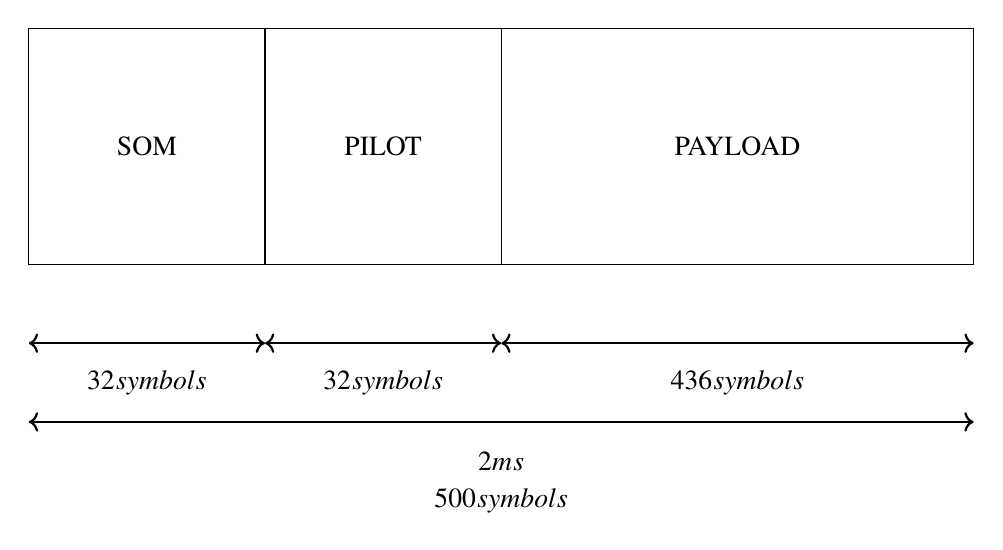
\begin{tikzpicture}


\draw (0,0) -- (12,0);
\draw (0,0) -- (0,-3) -- (12,-3) -- (12,0);
\draw (3,0) -- (3,-3);
\draw (6,0) -- (6,-3);


\node [align=center] at (1.5,-1.5) {SOM};
\node [align=center] at (4.5,-1.5) {PILOT};
\node [align=center] at (9,-1.5) {PAYLOAD};

\draw[<->,thick] (0,-4)--(3,-4) node[align = center] at (1.5,-4.5) {$32 symbols$};
\draw[<->,thick] (3,-4)--(6,-4) node[align = center] at (4.5,-4.5) {$32 symbols$};
\draw[<->,thick] (6,-4)--(12,-4) node[align = center] at (9,-4.5) {$436 symbols$};
\draw[<->,thick] (0,-5)--(12,-5) node[align = center] at (6,-5.5) {$2ms$};

\node [align=center] at (6,-6) {$500 symbols$};



\end{tikzpicture}
}
                \resizebox{\columnwidth}{!}{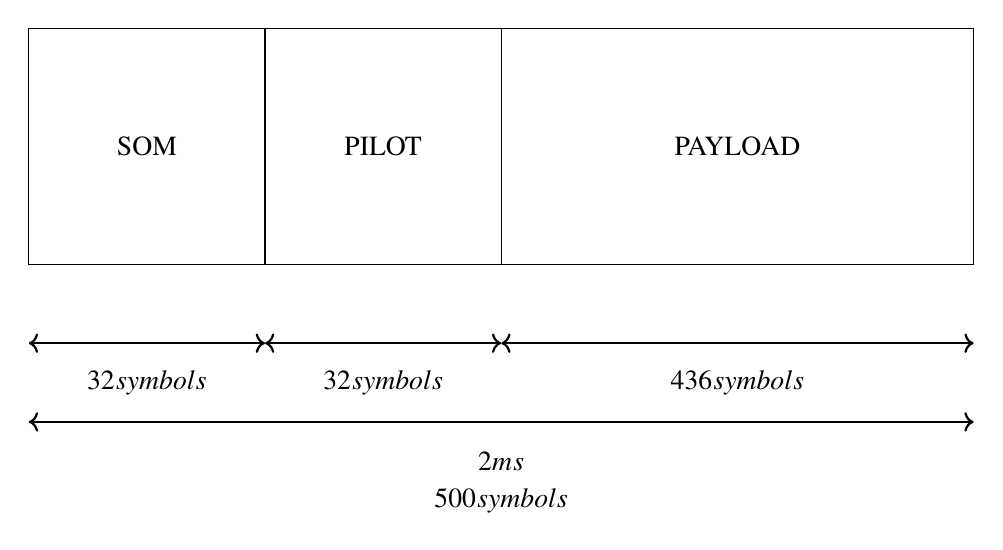
\begin{tikzpicture}


\draw (0,0) -- (12,0);
\draw (0,0) -- (0,-3) -- (12,-3) -- (12,0);
\draw (3,0) -- (3,-3);
\draw (6,0) -- (6,-3);


\node [align=center] at (1.5,-1.5) {SOM};
\node [align=center] at (4.5,-1.5) {PILOT};
\node [align=center] at (9,-1.5) {PAYLOAD};

\draw[<->,thick] (0,-4)--(3,-4) node[align = center] at (1.5,-4.5) {$32 symbols$};
\draw[<->,thick] (3,-4)--(6,-4) node[align = center] at (4.5,-4.5) {$32 symbols$};
\draw[<->,thick] (6,-4)--(12,-4) node[align = center] at (9,-4.5) {$436 symbols$};
\draw[<->,thick] (0,-5)--(12,-5) node[align = center] at (6,-5.5) {$2ms$};

\node [align=center] at (6,-6) {$500 symbols$};



\end{tikzpicture}
}
\caption{Physical Layer Frame}
\label{fig:ee18btech11041_frame}
\end{figure}
%\begin{table}[ht!]
%\centering
%%%%%%%%%%%%%%%%%%%%%%%%%%%%%%%%%%%%%%%%%%%%%%%%%%%%%%%%%%%%%%%%%%%%%%%
%%                                                                  %%
%%  This is the header of a LaTeX2e file exported from Gnumeric.    %%
%%                                                                  %%
%%  This file can be compiled as it stands or included in another   %%
%%  LaTeX document. The table is based on the longtable package so  %%
%%  the longtable options (headers, footers...) can be set in the   %%
%%  preamble section below (see PRAMBLE).                           %%
%%                                                                  %%
%%  To include the file in another, the following two lines must be %%
%%  in the including file:                                          %%
%%        \def\inputGnumericTable{}                                 %%
%%  at the beginning of the file and:                               %%
%%        \input{name-of-this-file.tex}                             %%
%%  where the table is to be placed. Note also that the including   %%
%%  file must use the following packages for the table to be        %%
%%  rendered correctly:                                             %%
%%    \usepackage[latin1]{inputenc}                                 %%
%%    \usepackage{color}                                            %%
%%    \usepackage{array}                                            %%
%%    \usepackage{longtable}                                        %%
%%    \usepackage{calc}                                             %%
%%    \usepackage{multirow}                                         %%
%%    \usepackage{hhline}                                           %%
%%    \usepackage{ifthen}                                           %%
%%  optionally (for landscape tables embedded in another document): %%
%%    \usepackage{lscape}                                           %%
%%                                                                  %%
%%%%%%%%%%%%%%%%%%%%%%%%%%%%%%%%%%%%%%%%%%%%%%%%%%%%%%%%%%%%%%%%%%%%%%



%%  This section checks if we are begin input into another file or  %%
%%  the file will be compiled alone. First use a macro taken from   %%
%%  the TeXbook ex 7.7 (suggestion of Han-Wen Nienhuys).            %%
\def\ifundefined#1{\expandafter\ifx\csname#1\endcsname\relax}


%%  Check for the \def token for inputed files. If it is not        %%
%%  defined, the file will be processed as a standalone and the     %%
%%  preamble will be used.                                          %%
\ifundefined{inputGnumericTable}

%%  We must be able to close or not the document at the end.        %%
	\def\gnumericTableEnd{\end{document}}


%%%%%%%%%%%%%%%%%%%%%%%%%%%%%%%%%%%%%%%%%%%%%%%%%%%%%%%%%%%%%%%%%%%%%%
%%                                                                  %%
%%  This is the PREAMBLE. Change these values to get the right      %%
%%  paper size and other niceties.                                  %%
%%                                                                  %%
%%%%%%%%%%%%%%%%%%%%%%%%%%%%%%%%%%%%%%%%%%%%%%%%%%%%%%%%%%%%%%%%%%%%%%

	\documentclass[12pt%
			  %,landscape%
                    ]{report}
       \usepackage[latin1]{inputenc}
       \usepackage{fullpage}
       \usepackage{color}
       \usepackage{array}
       \usepackage{longtable}
       \usepackage{calc}
       \usepackage{multirow}
       \usepackage{hhline}
       \usepackage{ifthen}

	\begin{document}


%%  End of the preamble for the standalone. The next section is for %%
%%  documents which are included into other LaTeX2e files.          %%
\else

%%  We are not a stand alone document. For a regular table, we will %%
%%  have no preamble and only define the closing to mean nothing.   %%
    \def\gnumericTableEnd{}

%%  If we want landscape mode in an embedded document, comment out  %%
%%  the line above and uncomment the two below. The table will      %%
%%  begin on a new page and run in landscape mode.                  %%
%       \def\gnumericTableEnd{\end{landscape}}
%       \begin{landscape}


%%  End of the else clause for this file being \input.              %%
\fi

%%%%%%%%%%%%%%%%%%%%%%%%%%%%%%%%%%%%%%%%%%%%%%%%%%%%%%%%%%%%%%%%%%%%%%
%%                                                                  %%
%%  The rest is the gnumeric table, except for the closing          %%
%%  statement. Changes below will alter the table's appearance.     %%
%%                                                                  %%
%%%%%%%%%%%%%%%%%%%%%%%%%%%%%%%%%%%%%%%%%%%%%%%%%%%%%%%%%%%%%%%%%%%%%%

\providecommand{\gnumericmathit}[1]{#1} 
%%  Uncomment the next line if you would like your numbers to be in %%
%%  italics if they are italizised in the gnumeric table.           %%
%\renewcommand{\gnumericmathit}[1]{\mathit{#1}}
\providecommand{\gnumericPB}[1]%
{\let\gnumericTemp=\\#1\let\\=\gnumericTemp\hspace{0pt}}
 \ifundefined{gnumericTableWidthDefined}
        \newlength{\gnumericTableWidth}
        \newlength{\gnumericTableWidthComplete}
        \newlength{\gnumericMultiRowLength}
        \global\def\gnumericTableWidthDefined{}
 \fi
%% The following setting protects this code from babel shorthands.  %%
 \ifthenelse{\isundefined{\languageshorthands}}{}{\languageshorthands{english}}
%%  The default table format retains the relative column widths of  %%
%%  gnumeric. They can easily be changed to c, r or l. In that case %%
%%  you may want to comment out the next line and uncomment the one %%
%%  thereafter                                                      %%
\providecommand\gnumbox{\makebox[0pt]}
%%\providecommand\gnumbox[1][]{\makebox}

%% to adjust positions in multirow situations                       %%
\setlength{\bigstrutjot}{\jot}
\setlength{\extrarowheight}{\doublerulesep}

%%  The \setlongtables command keeps column widths the same across  %%
%%  pages. Simply comment out next line for varying column widths.  %%
\setlongtables

\setlength\gnumericTableWidth{%
	70pt+%
	150pt+%
0pt}
\def\gumericNumCols{2}
\setlength\gnumericTableWidthComplete{\gnumericTableWidth+%
         \tabcolsep*\gumericNumCols*2+\arrayrulewidth*\gumericNumCols}
\ifthenelse{\lengthtest{\gnumericTableWidthComplete > \linewidth}}%
         {\def\gnumericScale{\ratio{\linewidth-%
                        \tabcolsep*\gumericNumCols*2-%
                        \arrayrulewidth*\gumericNumCols}%
{\gnumericTableWidth}}}%
{\def\gnumericScale{1}}

%%%%%%%%%%%%%%%%%%%%%%%%%%%%%%%%%%%%%%%%%%%%%%%%%%%%%%%%%%%%%%%%%%%%%%
%%                                                                  %%
%% The following are the widths of the various columns. We are      %%
%% defining them here because then they are easier to change.       %%
%% Depending on the cell formats we may use them more than once.    %%
%%                                                                  %%
%%%%%%%%%%%%%%%%%%%%%%%%%%%%%%%%%%%%%%%%%%%%%%%%%%%%%%%%%%%%%%%%%%%%%%

\ifthenelse{\isundefined{\gnumericColA}}{\newlength{\gnumericColA}}{}\settowidth{\gnumericColA}{\begin{tabular}{@{}p{70pt*\gnumericScale}@{}}x\end{tabular}}
\ifthenelse{\isundefined{\gnumericColB}}{\newlength{\gnumericColB}}{}\settowidth{\gnumericColB}{\begin{tabular}{@{}p{150pt*\gnumericScale}@{}}x\end{tabular}}

\begin{tabular}[c]{%
	b{\gnumericColA}%
	b{\gnumericColB}%
	}

%%%%%%%%%%%%%%%%%%%%%%%%%%%%%%%%%%%%%%%%%%%%%%%%%%%%%%%%%%%%%%%%%%%%%%
%%  The longtable options. (Caption, headers... see Goosens, p.124) %%
%	\caption{The Table Caption.}             \\	%
% \hline	% Across the top of the table.
%%  The rest of these options are table rows which are placed on    %%
%%  the first, last or every page. Use \multicolumn if you want.    %%

%%  Header for the first page.                                      %%
%	\multicolumn{2}{c}{The First Header} \\ \hline 
%	\multicolumn{1}{c}{colTag}	%Column 1
%	&\multicolumn{1}{c}{colTag}	\\ \hline %Last column
%	\endfirsthead

%%  The running header definition.                                  %%
%	\hline
%	\multicolumn{2}{l}{\ldots\small\slshape continued} \\ \hline
%	\multicolumn{1}{c}{colTag}	%Column 1
%	&\multicolumn{1}{c}{colTag}	\\ \hline %Last column
%	\endhead

%%  The running footer definition.                                  %%
%	\hline
%	\multicolumn{2}{r}{\small\slshape continued\ldots} \\
%	\endfoot

%%  The ending footer definition.                                   %%
%	\multicolumn{2}{c}{That's all folks} \\ \hline 
%	\endlastfoot
%%%%%%%%%%%%%%%%%%%%%%%%%%%%%%%%%%%%%%%%%%%%%%%%%%%%%%%%%%%%%%%%%%%%%%

\hhline{|-|-}
	 \multicolumn{1}{|p{\gnumericColA}|}%
	{\gnumericPB{\raggedright}\textbf{Parameter}}
	&\multicolumn{1}{p{\gnumericColB}|}%
	{\gnumericPB{\centering}\textbf{Value}}
\\
\hhline{|--|}
	 \multicolumn{1}{|p{\gnumericColA}|}%
	{\gnumericPB{\raggedright}Hardware}
	&\multicolumn{1}{p{\gnumericColB}|}%
	{\gnumericPB{\raggedleft}FPGA based baseband}
\\
\hhline{|--|}
	 \multicolumn{1}{|p{\gnumericColA}|}%
	{\gnumericPB{\raggedright}MODEM  }
	&\multicolumn{1}{p{\gnumericColB}|}%
	{\gnumericPB{\raggedleft}8PSK-TCM}
\\
\hhline{|--|}
	 \multicolumn{1}{|p{\gnumericColA}|}%
	{\gnumericPB{\raggedright}Modem Rate  }
	&\multicolumn{1}{p{\gnumericColB}|}%
	{\gnumericPB{\raggedleft}555Kbps}
\\
\hhline{|--|}
	 \multicolumn{1}{|p{\gnumericColA}|}%
	{\gnumericPB{\raggedright}SNR     }
	&\multicolumn{1}{p{\gnumericColB}|}%
	{\gnumericPB{\raggedleft}7.6 db at 1e5}
\\
\hhline{|--|}
	 \multicolumn{1}{|p{\gnumericColA}|}%
	{\gnumericPB{\raggedright}Channel  (V/UHF)}
	&\multicolumn{1}{p{\gnumericColB}|}%
	{\gnumericPB{\raggedleft}30Mhz - 512Mhz}
\\
\hhline{|--|}
	 \multicolumn{1}{|p{\gnumericColA}|}%
	{\gnumericPB{\raggedright}Bandwidth}
	&\multicolumn{1}{p{\gnumericColB}|}%
	{\gnumericPB{\raggedleft}250khz}
\\
\hhline{|--|}
	 \multicolumn{1}{|p{\gnumericColA}|}%
	{\gnumericPB{\raggedright}Bit Duration  }
	&\multicolumn{1}{p{\gnumericColB}|}%
	{\gnumericPB{\raggedleft}2.7us}
\\
\hhline{|--|}
	 \multicolumn{1}{|p{\gnumericColA}|}%
	{\gnumericPB{\raggedright}Throughput  }
	&\multicolumn{1}{p{\gnumericColB}|}%
	{\gnumericPB{\raggedleft}100kbps ( Throughput at application Layer)}
\\
\hhline{|--|}
	 \multicolumn{1}{|p{\gnumericColA}|}%
	{\gnumericPB{\raggedright}Ramp up time  }
	&\multicolumn{1}{p{\gnumericColB}|}%
	{\gnumericPB{\raggedleft}116 us (Junk symbols will be sent)}
\\
\hhline{|--|}
	 \multicolumn{1}{|p{\gnumericColA}|}%
	{\gnumericPB{\raggedright}Propagation Delay }
	&\multicolumn{1}{p{\gnumericColB}|}%
	{\gnumericPB{\raggedleft}100 us (Junk symbols will be sent)}
\\
\hhline{|--|}
	 \multicolumn{1}{|p{\gnumericColA}|}%
	{\gnumericPB{\raggedright}Training sequence }
	&\multicolumn{1}{p{\gnumericColB}|}%
	{\gnumericPB{\raggedleft}421.2us(provided time for training sequence)}
\\
\hhline{|--|}
	 \multicolumn{1}{|p{\gnumericColA}|}%
	{\gnumericPB{\raggedright}Frame Slot}
	&\multicolumn{1}{p{\gnumericColB}|}%
	{\gnumericPB{\raggedleft}2 ms}
\\
\hhline{|--|}
	 \multicolumn{1}{|p{\gnumericColA}|}%
	{\gnumericPB{\raggedright}Frame SOM}
	&\multicolumn{1}{p{\gnumericColB}|}%
	{\gnumericPB{\raggedleft}8 bytes}
\\
\hhline{|--|}
	 \multicolumn{1}{|p{\gnumericColA}|}%
	{\gnumericPB{\raggedright}Payload}
	&\multicolumn{1}{p{\gnumericColB}|}%
	{\gnumericPB{\raggedleft}32 bytes (692 us)}
\\
\hhline{|-|-|}
\end{tabular}

\ifthenelse{\isundefined{\languageshorthands}}{}{\languageshorthands{\languagename}}
\gnumericTableEnd

%\caption{Specifications}
%\label{table:specs}	
%\end{table}

\section{8-PSK}
\subsection{Modulation}
\begin{enumerate}[label=\thesubsection.\arabic*.,ref=\thesubsection.\theenumi]

\numberwithin{equation}{enumi}
\numberwithin{figure}{enumi}
\numberwithin{table}{enumi}


\item See Fig. \ref{fig:ee18btech11012_fig1} for the constellation diagram.  The transmitted symbol set is given by 
\begin{align}
\vec{s}_m = \myvec{\cos \frac{2m\pi}{8}\\ \sin \frac{2m\pi}{8}}, \quad m \in \cbrak{0,1,\dots,7}.
%\textbf{y = s + n}
\end{align}
%
The numerical values for $\vec{s}_m$ are listed in Table \ref{table:ee18btech11012_fig2}
\begin{figure}[!ht]
                \resizebox{\columnwidth}{!}{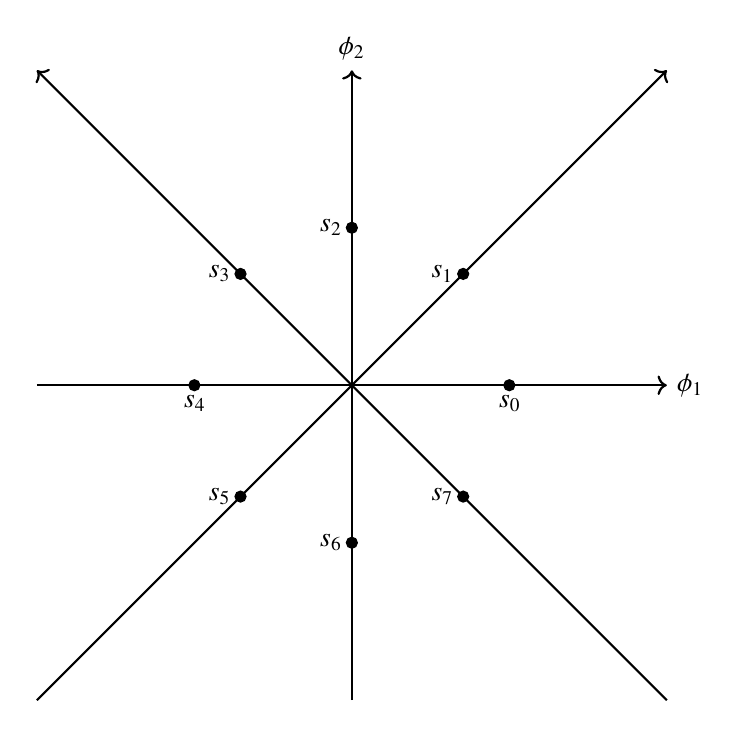
\begin{tikzpicture}

\draw[->,thick] (-4,0)--(4,0) node[right]{$\phi_1$};
\draw[->,thick] (0,-4)--(0,4) node[above]{$\phi_2$};
\draw[->,thick] (-4,-4)--(4,4) node[right]{};
\draw[->,thick] (4,-4)--(-4,4) node[above]{};

\filldraw[black] (2,0) circle (2pt) node[below] {$s_0$} ;
\filldraw[black] (1.414,1.414) circle (2pt) node[left] {$s_1$} ;
\filldraw[black] (0,2) circle (2pt) node[left] {$s_2$} ;
\filldraw[black] (-1.414,1.414) circle (2pt) node[left] {$s_3$} ;
\filldraw[black] (-2,0) circle (2pt) node[below] {$s_4$} ;
\filldraw[black] (-1.414,-1.414) circle (2pt) node[left] {$s_5$} ;
\filldraw[black] (0,-2) circle (2pt) node[left] {$s_6$} ;
\filldraw[black] (1.414,-1.414) circle (2pt) node[left] {$s_7$} ;


\end{tikzpicture}
}
\caption{Constellation diagram}
\label{fig:ee18btech11012_fig1}
\end{figure}


\item The gray code shown in Table \ref{table:ee18btech11012_fig2}
 is used for encoding the 8-PSK symbols.
\begin{table}[!ht]
                \resizebox{\columnwidth}{!}{%%%%%%%%%%%%%%%%%%%%%%%%%%%%%%%%%%%%%%%%%%%%%%%%%%%%%%%%%%%%%%%%%%%%%%
%%                                                                  %%
%%  This is the header of a LaTeX2e file exported from Gnumeric.    %%
%%                                                                  %%
%%  This file can be compiled as it stands or included in another   %%
%%  LaTeX document. The table is based on the longtable package so  %%
%%  the longtable options (headers, footers...) can be set in the   %%
%%  preamble section below (see PRAMBLE).                           %%
%%                                                                  %%
%%  To include the file in another, the following two lines must be %%
%%  in the including file:                                          %%
%%        \def\inputGnumericTable{}                                 %%
%%  at the beginning of the file and:                               %%
%%        \input{name-of-this-file.tex}                             %%
%%  where the table is to be placed. Note also that the including   %%
%%  file must use the following packages for the table to be        %%
%%  rendered correctly:                                             %%
%%    \usepackage[latin1]{inputenc}                                 %%
%%    \usepackage{color}                                            %%
%%    \usepackage{array}                                            %%
%%    \usepackage{longtable}                                        %%
%%    \usepackage{calc}                                             %%
%%    \usepackage{multirow}                                         %%
%%    \usepackage{hhline}                                           %%
%%    \usepackage{ifthen}                                           %%
%%  optionally (for landscape tables embedded in another document): %%
%%    \usepackage{lscape}                                           %%
%%                                                                  %%
%%%%%%%%%%%%%%%%%%%%%%%%%%%%%%%%%%%%%%%%%%%%%%%%%%%%%%%%%%%%%%%%%%%%%%



%%  This section checks if we are begin input into another file or  %%
%%  the file will be compiled alone. First use a macro taken from   %%
%%  the TeXbook ex 7.7 (suggestion of Han-Wen Nienhuys).            %%
\def\ifundefined#1{\expandafter\ifx\csname#1\endcsname\relax}


%%  Check for the \def token for inputed files. If it is not        %%
%%  defined, the file will be processed as a standalone and the     %%
%%  preamble will be used.                                          %%
\ifundefined{inputGnumericTable}

%%  We must be able to close or not the document at the end.        %%
	\def\gnumericTableEnd{\end{document}}


%%%%%%%%%%%%%%%%%%%%%%%%%%%%%%%%%%%%%%%%%%%%%%%%%%%%%%%%%%%%%%%%%%%%%%
%%                                                                  %%
%%  This is the PREAMBLE. Change these values to get the right      %%
%%  paper size and other niceties.                                  %%
%%                                                                  %%
%%%%%%%%%%%%%%%%%%%%%%%%%%%%%%%%%%%%%%%%%%%%%%%%%%%%%%%%%%%%%%%%%%%%%%

	\documentclass[12pt%
			  %,landscape%
                    ]{report}
       \usepackage[latin1]{inputenc}
       \usepackage{fullpage}
       \usepackage{color}
       \usepackage{array}
       \usepackage{longtable}
       \usepackage{calc}
       \usepackage{multirow}
       \usepackage{hhline}
       \usepackage{ifthen}

	\begin{document}


%%  End of the preamble for the standalone. The next section is for %%
%%  documents which are included into other LaTeX2e files.          %%
\else

%%  We are not a stand alone document. For a regular table, we will %%
%%  have no preamble and only define the closing to mean nothing.   %%
    \def\gnumericTableEnd{}

%%  If we want landscape mode in an embedded document, comment out  %%
%%  the line above and uncomment the two below. The table will      %%
%%  begin on a new page and run in landscape mode.                  %%
%       \def\gnumericTableEnd{\end{landscape}}
%       \begin{landscape}


%%  End of the else clause for this file being \input.              %%
\fi

%%%%%%%%%%%%%%%%%%%%%%%%%%%%%%%%%%%%%%%%%%%%%%%%%%%%%%%%%%%%%%%%%%%%%%
%%                                                                  %%
%%  The rest is the gnumeric table, except for the closing          %%
%%  statement. Changes below will alter the table's appearance.     %%
%%                                                                  %%
%%%%%%%%%%%%%%%%%%%%%%%%%%%%%%%%%%%%%%%%%%%%%%%%%%%%%%%%%%%%%%%%%%%%%%

\providecommand{\gnumericmathit}[1]{#1} 
%%  Uncomment the next line if you would like your numbers to be in %%
%%  italics if they are italizised in the gnumeric table.           %%
%\renewcommand{\gnumericmathit}[1]{\mathit{#1}}
\providecommand{\gnumericPB}[1]%
{\let\gnumericTemp=\\#1\let\\=\gnumericTemp\hspace{0pt}}
 \ifundefined{gnumericTableWidthDefined}
        \newlength{\gnumericTableWidth}
        \newlength{\gnumericTableWidthComplete}
        \newlength{\gnumericMultiRowLength}
        \global\def\gnumericTableWidthDefined{}
 \fi
%% The following setting protects this code from babel shorthands.  %%
 \ifthenelse{\isundefined{\languageshorthands}}{}{\languageshorthands{english}}
%%  The default table format retains the relative column widths of  %%
%%  gnumeric. They can easily be changed to c, r or l. In that case %%
%%  you may want to comment out the next line and uncomment the one %%
%%  thereafter                                                      %%
\providecommand\gnumbox{\makebox[0pt]}
%%\providecommand\gnumbox[1][]{\makebox}

%% to adjust positions in multirow situations                       %%
\setlength{\bigstrutjot}{\jot}
\setlength{\extrarowheight}{\doublerulesep}

%%  The \setlongtables command keeps column widths the same across  %%
%%  pages. Simply comment out next line for varying column widths.  %%
\setlongtables

\setlength\gnumericTableWidth{%
	71pt+%
	53pt+%
	69pt+%
0pt}
\def\gumericNumCols{3}
\setlength\gnumericTableWidthComplete{\gnumericTableWidth+%
         \tabcolsep*\gumericNumCols*2+\arrayrulewidth*\gumericNumCols}
\ifthenelse{\lengthtest{\gnumericTableWidthComplete > \linewidth}}%
         {\def\gnumericScale{\ratio{\linewidth-%
                        \tabcolsep*\gumericNumCols*2-%
                        \arrayrulewidth*\gumericNumCols}%
{\gnumericTableWidth}}}%
{\def\gnumericScale{1}}

%%%%%%%%%%%%%%%%%%%%%%%%%%%%%%%%%%%%%%%%%%%%%%%%%%%%%%%%%%%%%%%%%%%%%%
%%                                                                  %%
%% The following are the widths of the various columns. We are      %%
%% defining them here because then they are easier to change.       %%
%% Depending on the cell formats we may use them more than once.    %%
%%                                                                  %%
%%%%%%%%%%%%%%%%%%%%%%%%%%%%%%%%%%%%%%%%%%%%%%%%%%%%%%%%%%%%%%%%%%%%%%

\ifthenelse{\isundefined{\gnumericColA}}{\newlength{\gnumericColA}}{}\settowidth{\gnumericColA}{\begin{tabular}{@{}p{71pt*\gnumericScale}@{}}x\end{tabular}}
\ifthenelse{\isundefined{\gnumericColB}}{\newlength{\gnumericColB}}{}\settowidth{\gnumericColB}{\begin{tabular}{@{}p{53pt*\gnumericScale}@{}}x\end{tabular}}
\ifthenelse{\isundefined{\gnumericColC}}{\newlength{\gnumericColC}}{}\settowidth{\gnumericColC}{\begin{tabular}{@{}p{69pt*\gnumericScale}@{}}x\end{tabular}}

\begin{tabular}[c]{%
	b{\gnumericColA}%
	b{\gnumericColB}%
	b{\gnumericColC}%
	}

%%%%%%%%%%%%%%%%%%%%%%%%%%%%%%%%%%%%%%%%%%%%%%%%%%%%%%%%%%%%%%%%%%%%%%
%%  The longtable options. (Caption, headers... see Goosens, p.124) %%
%	\caption{The Table Caption.}             \\	%
% \hline	% Across the top of the table.
%%  The rest of these options are table rows which are placed on    %%
%%  the first, last or every page. Use \multicolumn if you want.    %%

%%  Header for the first page.                                      %%
%	\multicolumn{3}{c}{The First Header} \\ \hline 
%	\multicolumn{1}{c}{colTag}	%Column 1
%	&\multicolumn{1}{c}{colTag}	%Column 2
%	&\multicolumn{1}{c}{colTag}	\\ \hline %Last column
%	\endfirsthead

%%  The running header definition.                                  %%
%	\hline
%	\multicolumn{3}{l}{\ldots\small\slshape continued} \\ \hline
%	\multicolumn{1}{c}{colTag}	%Column 1
%	&\multicolumn{1}{c}{colTag}	%Column 2
%	&\multicolumn{1}{c}{colTag}	\\ \hline %Last column
%	\endhead

%%  The running footer definition.                                  %%
%	\hline
%	\multicolumn{3}{r}{\small\slshape continued\ldots} \\
%	\endfoot

%%  The ending footer definition.                                   %%
%	\multicolumn{3}{c}{That's all folks} \\ \hline 
%	\endlastfoot
%%%%%%%%%%%%%%%%%%%%%%%%%%%%%%%%%%%%%%%%%%%%%%%%%%%%%%%%%%%%%%%%%%%%%%
\hhline{|-|-|-}
	 \multicolumn{1}{|p{\gnumericColA}|}%
	{\gnumericPB{\centering}\gnumbox{Symbol}}
	&\multicolumn{1}{p{\gnumericColB}|}%
	{\gnumericPB{\centering}\gnumbox{Gray Code}}
	&\multicolumn{1}{p{\gnumericColC}|}%
	{\gnumericPB{\centering}\gnumbox{Value}}
\\
\hhline{|---|}
	 \multicolumn{1}{|p{\gnumericColA}|}%
	{\gnumericPB{\centering}\gnumbox{$s_0$}}
	&\multicolumn{1}{p{\gnumericColB}|}%
	{\gnumericPB{\centering}\gnumbox{000}}
	&\multicolumn{1}{p{\gnumericColC}|}%
	{\gnumericPB{\centering}\gnumbox{\myvec{1\\0 }}}
\\
\hhline{|---|}
	 \multicolumn{1}{|p{\gnumericColA}|}%
	{\gnumericPB{\centering}\gnumbox{$s_1$}}
	&\multicolumn{1}{p{\gnumericColB}|}%
	{\gnumericPB{\centering}\gnumbox{001}}
	&\multicolumn{1}{p{\gnumericColC}|}%
	{\gnumericPB{\centering}\gnumbox{\myvec{\frac{1}{\sqrt{2}}\\\frac{1}{\sqrt{2}}}}}
\\
\hhline{|---|}
	 \multicolumn{1}{|p{\gnumericColA}|}%
	{\gnumericPB{\centering}\gnumbox{$s_2$}}
	&\multicolumn{1}{p{\gnumericColB}|}%
	{\gnumericPB{\centering}\gnumbox{011}}
	&\multicolumn{1}{p{\gnumericColC}|}%
	{\gnumericPB{\centering}\gnumbox{\myvec{0\\1}}}
\\
\hhline{|---|}
	 \multicolumn{1}{|p{\gnumericColA}|}%
	{\gnumericPB{\centering}\gnumbox{$s_3$}}
	&\multicolumn{1}{p{\gnumericColB}|}%
	{\gnumericPB{\centering}\gnumbox{010}}
	&\multicolumn{1}{p{\gnumericColC}|}%
	{\gnumericPB{\centering}\gnumbox{\myvec{\frac{-1}{\sqrt{2}}\\\frac{1}{\sqrt{2}}}}}
\\
\hhline{|---|}
	 \multicolumn{1}{|p{\gnumericColA}|}%
	{\gnumericPB{\centering}\gnumbox{$s_4$}}
	&\multicolumn{1}{p{\gnumericColB}|}%
	{\gnumericPB{\centering}\gnumbox{110}}
	&\multicolumn{1}{p{\gnumericColC}|}%
	{\gnumericPB{\centering}\gnumbox{\myvec{-1\\0}}}
\\
\hhline{|---|}
	 \multicolumn{1}{|p{\gnumericColA}|}%
	{\gnumericPB{\centering}\gnumbox{$s_5$}}
	&\multicolumn{1}{p{\gnumericColB}|}%
	{\gnumericPB{\centering}\gnumbox{111}}
	&\multicolumn{1}{p{\gnumericColC}|}%
	{\gnumericPB{\centering}\gnumbox{\myvec{\frac{-1}{\sqrt{2}}\\\frac{-1}{\sqrt{2}}}}}
\\
\hhline{|---|}
	 \multicolumn{1}{|p{\gnumericColA}|}%
	{\gnumericPB{\centering}\gnumbox{$s_6$}}
	&\multicolumn{1}{p{\gnumericColB}|}%
	{\gnumericPB{\centering}\gnumbox{101}}
	&\multicolumn{1}{p{\gnumericColC}|}%
	{\gnumericPB{\centering}\gnumbox{\myvec{0\\-1}}}
\\
\hhline{|---|}
	 \multicolumn{1}{|p{\gnumericColA}|}%
	{\gnumericPB{\centering}\gnumbox{$s_7$}}
	&\multicolumn{1}{p{\gnumericColB}|}%
	{\gnumericPB{\centering}\gnumbox{100}}
	&\multicolumn{1}{p{\gnumericColC}|}%
	{\gnumericPB{\centering}\gnumbox{\myvec{\frac{1}{\sqrt{2}}\\\frac{-1}{\sqrt{2}}}}}
\\
\hhline{|-|-|-|}
\end{tabular}


\ifthenelse{\isundefined{\languageshorthands}}{}{\languageshorthands{\languagename}}
\gnumericTableEnd
}
\caption{Gray coding}
\label{table:ee18btech11012_fig2}
\end{table}

%$s_0$ denote bits 000, $s_1$ denote bits 001, $s_2$ denote bits 011,$s_3$ denote bits 010,$s_4$ denote bits 110,$s_5$ denote bits 111,$s_6$ denote bits 101,$s_7$ denote bits 100.

\item The received symbol is then obtained as
\begin{align}
\vec{y} = \sqrt{E_s}\vec{s} + \vec{n}
\end{align}
%
where $E_s$ is the symbol energy and 

\begin{align}
\vec{n} &\sim \mathcal{N}\brak{\vec{0},\frac{N_0}{2}\vec{I}}
\\
\vec{s} &\in \cbrak{\vec{s}_m}_{m = 0}^{7}
\end{align}

\item Using the ML criterion, the decision rule for each symbol is given by Fig. \ref{fig:ee18btech11012_fig2}.  For $\vec{s}_0$, this can be expressed as
\begin{align}
    \norm{\textbf{y}-\textbf{$s_{0}$}}^2 & \le \norm{\textbf{y}-\textbf{$s_{i}$}}^2, \quad i = 1,\dots,7\\
\implies \brak{\vec{s}_0 - \vec{s}_i}^T \vec{y} &\ge 0\\
%    \norm{\textbf{y}-\textbf{$s_{0}$}}^2 &< \norm{\textbf{y}-\textbf{$s_{1}$}}^2\\
%    \norm{\textbf{y}-\textbf{$s_{0}$}}^2 &< \norm{\textbf{y}-\textbf{$s_{2}$}}^2\\
%    \norm{\textbf{y}-\textbf{$s_{0}$}}^2 &< \norm{\textbf{y}-\textbf{$s_{3}$}}^2\\
%    \norm{\textbf{y}-\textbf{$s_{0}$}}^2 &< \norm{\textbf{y}-\textbf{$s_{4}$}}^2\\
%    \norm{\textbf{y}-\textbf{$s_{0}$}}^2 &< \norm{\textbf{y}-\textbf{$s_{5}$}}^2\\
%    \norm{\textbf{y}-\textbf{$s_{0}$}}^2 &< \norm{\textbf{y}-\textbf{$s_{6}$}}^2\\
%    \norm{\textbf{y}-\textbf{$s_{0}$}}^2 &< \norm{\textbf{y}-\textbf{$s_{7}$}}^2
\end{align}
%
which can be simplified to obtain the matrix inequality
\begin{align}
\myvec{
\brak{\vec{s}_0 - \vec{s}_1}^T \\
\brak{\vec{s}_0 - \vec{s}_2}^T\\
\brak{\vec{s}_0 - \vec{s}_3}^T\\
\brak{\vec{s}_0 - \vec{s}_4}^T\\
\brak{\vec{s}_0 - \vec{s}_5}^T\\
\brak{\vec{s}_0 - \vec{s}_6}^T\\
\brak{\vec{s}_0 - \vec{s}_7}^T
}\vec{y} \succeq \vec{0} 
%    (s_{0}-s_{1})^Ty>0
%    (s_{0}-s_{2})^Ty>0
%    (s_{0}-s_{3})^Ty>0
%    (s_{0}-s_{4})^Ty>0
%    (s_{0}-s_{5})^Ty>0
%    (s_{0}-s_{6})^Ty>0
%    (s_{0}-s_{7})^Ty>0
\end{align}
%
resulting in 
\begin{align}
\myvec{\sqrt{2} - 1 & 1 \\ \sqrt{2} - 1 & -1} \vec{y} \succeq \vec{0}
\end{align}

\begin{figure}[!ht]

                \resizebox{\columnwidth}{!}{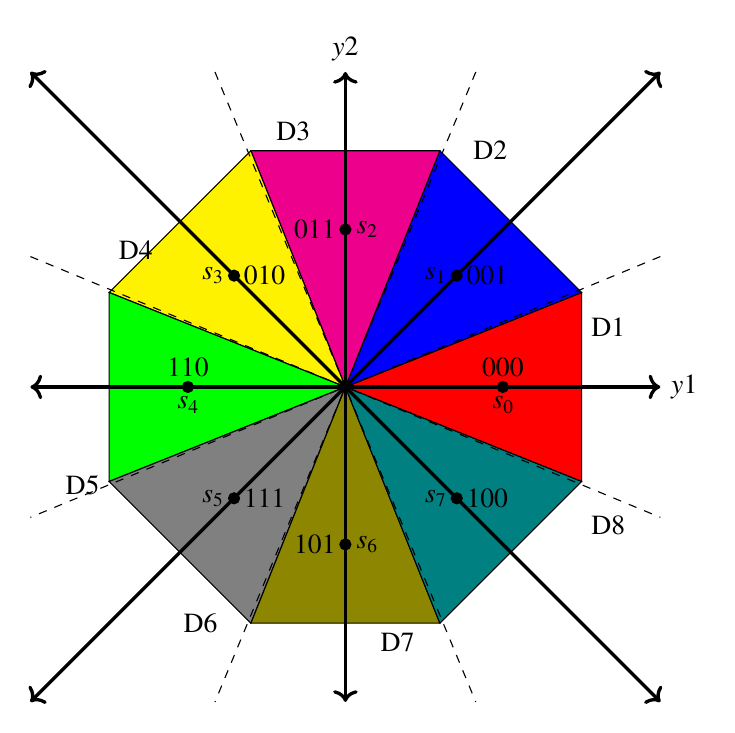
\begin{tikzpicture}
\draw[fill=red]  (0,0) -- (3,1.2) -- (3,-1.2) -- (0,0) -- cycle;
\draw[fill=blue]  (0,0) -- (1.2,3) -- (3,1.2) -- (0,0) -- cycle;
\draw[fill=magenta!100]  (0,0) -- (-1.2,3) -- (1.2,3) -- (0,0) -- cycle;
\draw[fill=yellow]  (0,0) -- (-1.2,3) -- (-3,1.2) -- (0,0) -- cycle;
\draw[fill=green]  (0,0) -- (-3,1.2) -- (-3,-1.2) -- (0,0) -- cycle;
\draw[fill=gray]  (0,0) -- (-3,-1.2) -- (-1.2,-3) -- (0,0) -- cycle;
\draw[fill=olive]  (0,0) -- (-1.2,-3) -- (1.2,-3) -- (0,0) -- cycle;
\draw[fill=teal]  (0,0) -- (1.2,-3) -- (3,-1.2) -- (0,0) -- cycle;
\draw[<->,very thick] (-4,0)--(4,0) node[right]{$y1$};
\draw[<->,very thick] (0,-4)--(0,4) node[above]{$y2$};
\draw[dashed] (4,1.656)--(-4,-1.656);
\draw[dashed] (1.656,4)--(-1.656,-4);
\draw[dashed] (-1.656,4)--(1.656,-4);
\draw[dashed] (-4,1.656)--(4,-1.656);
\draw[<->,very thick](-4,-4)--(4,4);
\draw[<->,very thick](-4,4)--(4,-4);

\filldraw[black] (2,0) circle (2pt) node[below] {$s_0$} node[above] {000};
\filldraw[black] (1.414,1.414) circle (2pt) node[left] {$s_1$} node[right] {001};
\filldraw[black] (0,2) circle (2pt) node[right] {$s_2$} node[left] {011};
\filldraw[black] (-1.414,1.414) circle (2pt) node[left] {$s_3$} node [right] {010};
\filldraw[black] (-2,0) circle (2pt) node[below] {$s_4$} node[above] {110};
\filldraw[black] (-1.414,-1.414) circle (2pt) node[left] {$s_5$} node[right] {111};
\filldraw[black] (0,-2) circle (2pt) node[right] {$s_6$} node[left] {101};
\filldraw[black] (1.414,-1.414) circle (2pt) node[left] {$s_7$} node [right] {100};

\foreach \coordinate/\label/\pos in {{(3,1)/D1/below right},{(1.5,3)/D2/right},{(-1,3)/D3/above right},{(-3,1.5)/D4/above right},{(-3,-1.5)/D5/above left},{(-1.5,-3)/D6/left},{(1,-3)/D7/below left},{(3,-2)/D8/above right}} \node[\pos] at \coordinate {\label};

\end{tikzpicture}
}

\caption{decision regions}
\label{fig:ee18btech11012_fig2}
	
\end{figure}

%\begin{figure}[!ht]
%
%                \resizebox{\columnwidth}{!}{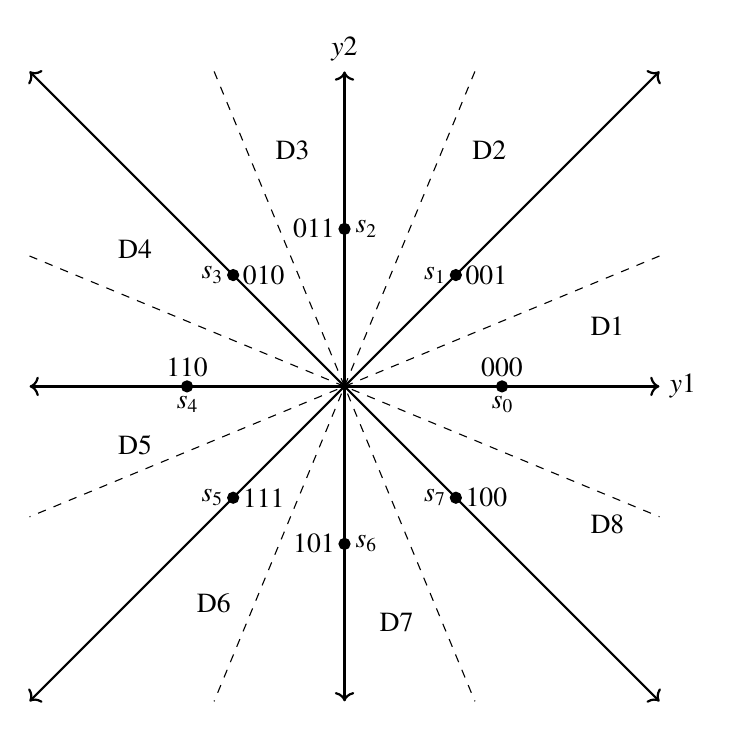
\begin{tikzpicture}

\draw[<->,thick] (-4,0)--(4,0) node[right]{$y1$};
\draw[<->,thick] (0,-4)--(0,4) node[above]{$y2$};
\draw[dashed] (4,1.656)--(-4,-1.656);
\draw[dashed] (1.656,4)--(-1.656,-4);
\draw[dashed] (-1.656,4)--(1.656,-4);
\draw[dashed] (-4,1.656)--(4,-1.656);
\draw[<->,thick](-4,-4)--(4,4);
\draw[<->,thick](-4,4)--(4,-4);

\filldraw[black] (2,0) circle (2pt) node[below] {$s_0$} node[above] {000};
\filldraw[black] (1.414,1.414) circle (2pt) node[left] {$s_1$} node[right] {001};
\filldraw[black] (0,2) circle (2pt) node[right] {$s_2$} node[left] {011};
\filldraw[black] (-1.414,1.414) circle (2pt) node[left] {$s_3$} node [right] {010};
\filldraw[black] (-2,0) circle (2pt) node[below] {$s_4$} node[above] {110};
\filldraw[black] (-1.414,-1.414) circle (2pt) node[left] {$s_5$} node[right] {111};
\filldraw[black] (0,-2) circle (2pt) node[right] {$s_6$} node[left] {101};
\filldraw[black] (1.414,-1.414) circle (2pt) node[left] {$s_7$} node [right] {100};

\foreach \coordinate/\label/\pos in {{(3,1)/D1/below right},{(1.5,3)/D2/right},{(-1,3)/D3/right},{(-3,1.5)/D4/above right},{(-3,-1)/D5/above right},{(-2,-3)/D6/above right},{(1,-3)/D7/left},{(3,-2)/D8/above right}} \node[\pos] at \coordinate {\label};

\end{tikzpicture}
}
%
%\label{fig:ee18btech11012_fig2}
%\caption{decision regions}
%	
%\end{figure}



Similarly the decisions for all symbols 
are available in Table \ref{table:ee18btech11012_fig4}
%
\begin{table}[!ht]
                \resizebox{\columnwidth}{!}{%%%%%%%%%%%%%%%%%%%%%%%%%%%%%%%%%%%%%%%%%%%%%%%%%%%%%%%%%%%%%%%%%%%%%%
%%                                                                  %%
%%  This is the header of a LaTeX2e file exported from Gnumeric.    %%
%%                                                                  %%
%%  This file can be compiled as it stands or included in another   %%
%%  LaTeX document. The table is based on the longtable package so  %%
%%  the longtable options (headers, footers...) can be set in the   %%
%%  preamble section below (see PRAMBLE).                           %%
%%                                                                  %%
%%  To include the file in another, the following two lines must be %%
%%  in the including file:                                          %%
%%        \def\inputGnumericTable{}                                 %%
%%  at the beginning of the file and:                               %%
%%        \input{name-of-this-file.tex}                             %%
%%  where the table is to be placed. Note also that the including   %%
%%  file must use the following packages for the table to be        %%
%%  rendered correctly:                                             %%
%%    \usepackage[latin1]{inputenc}                                 %%
%%    \usepackage{color}                                            %%
%%    \usepackage{array}                                            %%
%%    \usepackage{longtable}                                        %%
%%    \usepackage{calc}                                             %%
%%    \usepackage{multirow}                                         %%
%%    \usepackage{hhline}                                           %%
%%    \usepackage{ifthen}                                           %%
%%  optionally (for landscape tables embedded in another document): %%
%%    \usepackage{lscape}                                           %%
%%                                                                  %%
%%%%%%%%%%%%%%%%%%%%%%%%%%%%%%%%%%%%%%%%%%%%%%%%%%%%%%%%%%%%%%%%%%%%%%



%%  This section checks if we are begin input into another file or  %%
%%  the file will be compiled alone. First use a macro taken from   %%
%%  the TeXbook ex 7.7 (suggestion of Han-Wen Nienhuys).            %%
\def\ifundefined#1{\expandafter\ifx\csname#1\endcsname\relax}


%%  Check for the \def token for inputed files. If it is not        %%
%%  defined, the file will be processed as a standalone and the     %%
%%  preamble will be used.                                          %%
\ifundefined{inputGnumericTable}

%%  We must be able to close or not the document at the end.        %%
	\def\gnumericTableEnd{\end{document}}


%%%%%%%%%%%%%%%%%%%%%%%%%%%%%%%%%%%%%%%%%%%%%%%%%%%%%%%%%%%%%%%%%%%%%%
%%                                                                  %%
%%  This is the PREAMBLE. Change these values to get the right      %%
%%  paper size and other niceties.                                  %%
%%                                                                  %%
%%%%%%%%%%%%%%%%%%%%%%%%%%%%%%%%%%%%%%%%%%%%%%%%%%%%%%%%%%%%%%%%%%%%%%

	\documentclass[12pt%
			  %,landscape%
                    ]{report}
       \usepackage[latin1]{inputenc}
       \usepackage{fullpage}
       \usepackage{color}
       \usepackage{array}
       \usepackage{longtable}
       \usepackage{calc}
       \usepackage{multirow}
       \usepackage{hhline}
       \usepackage{ifthen}

	\begin{document}


%%  End of the preamble for the standalone. The next section is for %%
%%  documents which are included into other LaTeX2e files.          %%
\else

%%  We are not a stand alone document. For a regular table, we will %%
%%  have no preamble and only define the closing to mean nothing.   %%
    \def\gnumericTableEnd{}

%%  If we want landscape mode in an embedded document, comment out  %%
%%  the line above and uncomment the two below. The table will      %%
%%  begin on a new page and run in landscape mode.                  %%
%       \def\gnumericTableEnd{\end{landscape}}
%       \begin{landscape}


%%  End of the else clause for this file being \input.              %%
\fi

%%%%%%%%%%%%%%%%%%%%%%%%%%%%%%%%%%%%%%%%%%%%%%%%%%%%%%%%%%%%%%%%%%%%%%
%%                                                                  %%
%%  The rest is the gnumeric table, except for the closing          %%
%%  statement. Changes below will alter the table's appearance.     %%
%%                                                                  %%
%%%%%%%%%%%%%%%%%%%%%%%%%%%%%%%%%%%%%%%%%%%%%%%%%%%%%%%%%%%%%%%%%%%%%%

\providecommand{\gnumericmathit}[1]{#1} 
%%  Uncomment the next line if you would like your numbers to be in %%
%%  italics if they are italizised in the gnumeric table.           %%
%\renewcommand{\gnumericmathit}[1]{\mathit{#1}}
\providecommand{\gnumericPB}[1]%
{\let\gnumericTemp=\\#1\let\\=\gnumericTemp\hspace{0pt}}
 \ifundefined{gnumericTableWidthDefined}
        \newlength{\gnumericTableWidth}
        \newlength{\gnumericTableWidthComplete}
        \newlength{\gnumericMultiRowLength}
        \global\def\gnumericTableWidthDefined{}
 \fi
%% The following setting protects this code from babel shorthands.  %%
 \ifthenelse{\isundefined{\languageshorthands}}{}{\languageshorthands{english}}
%%  The default table format retains the relative column widths of  %%
%%  gnumeric. They can easily be changed to c, r or l. In that case %%
%%  you may want to comment out the next line and uncomment the one %%
%%  thereafter                                                      %%
\providecommand\gnumbox{\makebox[0pt]}
%%\providecommand\gnumbox[1][]{\makebox}

%% to adjust positions in multirow situations                       %%
\setlength{\bigstrutjot}{\jot}
\setlength{\extrarowheight}{\doublerulesep}

%%  The \setlongtables command keeps column widths the same across  %%
%%  pages. Simply comment out next line for varying column widths.  %%
\setlongtables

\setlength\gnumericTableWidth{%
	71pt+%
	53pt+%
	73pt+%
0pt}
\def\gumericNumCols{3}
\setlength\gnumericTableWidthComplete{\gnumericTableWidth+%
         \tabcolsep*\gumericNumCols*2+\arrayrulewidth*\gumericNumCols}
\ifthenelse{\lengthtest{\gnumericTableWidthComplete > \linewidth}}%
         {\def\gnumericScale{\ratio{\linewidth-%
                        \tabcolsep*\gumericNumCols*2-%
                        \arrayrulewidth*\gumericNumCols}%
{\gnumericTableWidth}}}%
{\def\gnumericScale{1}}

%%%%%%%%%%%%%%%%%%%%%%%%%%%%%%%%%%%%%%%%%%%%%%%%%%%%%%%%%%%%%%%%%%%%%%
%%                                                                  %%
%% The following are the widths of the various columns. We are      %%
%% defining them here because then they are easier to change.       %%
%% Depending on the cell formats we may use them more than once.    %%
%%                                                                  %%
%%%%%%%%%%%%%%%%%%%%%%%%%%%%%%%%%%%%%%%%%%%%%%%%%%%%%%%%%%%%%%%%%%%%%%

\ifthenelse{\isundefined{\gnumericColA}}{\newlength{\gnumericColA}}{}\settowidth{\gnumericColA}{\begin{tabular}{@{}p{40pt*\gnumericScale}@{}}x\end{tabular}}
\ifthenelse{\isundefined{\gnumericColB}}{\newlength{\gnumericColB}}{}\settowidth{\gnumericColB}{\begin{tabular}{@{}p{71pt*\gnumericScale}@{}}x\end{tabular}}
\ifthenelse{\isundefined{\gnumericColC}}{\newlength{\gnumericColC}}{}\settowidth{\gnumericColC}{\begin{tabular}{@{}p{205pt*\gnumericScale}@{}}x\end{tabular}}
\ifthenelse{\isundefined{\gnumericColD}}{\newlength{\gnumericColD}}{}\settowidth{\gnumericColD}{\begin{tabular}{@{}p{200pt*\gnumericScale}@{}}x\end{tabular}}

\begin{tabular}[c]{%
	b{\gnumericColA}%
	b{\gnumericColB}%
	b{\gnumericColC}%
	b{\gnumericColD}%
	}

%%%%%%%%%%%%%%%%%%%%%%%%%%%%%%%%%%%%%%%%%%%%%%%%%%%%%%%%%%%%%%%%%%%%%%
%%  The longtable options. (Caption, headers... see Goosens, p.124) %%
%	\caption{The Table Caption.}             \\	%
% \hline	% Across the top of the table.
%%  The rest of these options are table rows which are placed on    %%
%%  the first, last or every page. Use \multicolumn if you want.    %%

%%  Header for the first page.                                      %%
%	\multicolumn{3}{c}{The First Header} \\ \hline 
%	\multicolumn{1}{c}{colTag}	%Column 1
%	&\multicolumn{1}{c}{colTag}	%Column 2
%	&\multicolumn{1}{c}{colTag}	\\ \hline %Last column
%	\endfirsthead

%%  The running header definition.                                  %%
%	\hline
%	\multicolumn{3}{l}{\ldots\small\slshape continued} \\ \hline
%	\multicolumn{1}{c}{colTag}	%Column 1
%	&\multicolumn{1}{c}{colTag}	%Column 2
%	&\multicolumn{1}{c}{colTag}	\\ \hline %Last column
%	\endhead

%%  The running footer definition.                                  %%
%	\hline
%	\multicolumn{3}{r}{\small\slshape continued\ldots} \\
%	\endfoot

%%  The ending footer definition.                                   %%
%	\multicolumn{3}{c}{That's all folks} \\ \hline 
%	\endlastfoot
%%%%%%%%%%%%%%%%%%%%%%%%%%%%%%%%%%%%%%%%%%%%%%%%%%%%%%%%%%%%%%%%%%%%%%
\hhline{|-|-|-|-}
	 \multicolumn{1}{|p{\gnumericColA}|}%
	{\gnumericPB{\centering}\gnumbox{Symbol}}
	&\multicolumn{1}{p{\gnumericColB}|}%
	{\gnumericPB{\centering}\gnumbox{Decision region}}
	&\multicolumn{1}{p{\gnumericColC}|}%
	{\gnumericPB{\centering}\gnumbox{Inequality}}
	&\multicolumn{1}{p{\gnumericColD}|}%
	{\gnumericPB{\centering}\gnumbox{Matrix Inequality}}
\\
\hhline{|----|}
	 \multicolumn{1}{|p{\gnumericColA}|}%
	{\gnumericPB{\centering}\gnumbox{$\vec{s}_0$}}
	&\multicolumn{1}{p{\gnumericColB}|}%
	{\gnumericPB{\centering}\gnumbox{D1}}
	&\multicolumn{1}{p{\gnumericColC}|}%
	{\gnumericPB{\centering}\gnumbox{$y_2+(\sqrt{2}-1)y_1>0$, $y_2-(\sqrt{2}-1)y_1<0$}}
	&\multicolumn{1}{p{\gnumericColD}|}%
	{\gnumericPB{\centering}\gnumbox{${\myvec{\sqrt{2}-1 & 1 \\ \sqrt{2}-1 & -1 }\vec{y}\succeq \vec{0}}$}}
\\
\hhline{|----|}
	 \multicolumn{1}{|p{\gnumericColA}|}%
	{\gnumericPB{\centering}\gnumbox{$\vec{s}_1$}}
	&\multicolumn{1}{p{\gnumericColB}|}%
	{\gnumericPB{\centering}\gnumbox{D2}}
	&\multicolumn{1}{p{\gnumericColC}|}%
	{\gnumericPB{\centering}\gnumbox{$y_2-(\sqrt{2}+1)y_1<0$, $y_2-(\sqrt{2}-1)y_1>0$}}
	&\multicolumn{1}{p{\gnumericColD}|}%
	{\gnumericPB{\centering}\gnumbox{${\myvec{\sqrt{2}+1 & -1 \\ -(\sqrt{2}-1) & 1}\vec{y}\succeq \vec{0}}$}}
\\
\hhline{|----|}
	 \multicolumn{1}{|p{\gnumericColA}|}%
	{\gnumericPB{\centering}\gnumbox{$\vec{s}_2$}}
	&\multicolumn{1}{p{\gnumericColB}|}%
	{\gnumericPB{\centering}\gnumbox{D3}}
	&\multicolumn{1}{p{\gnumericColC}|}%
	{\gnumericPB{\centering}\gnumbox{$y_2-(\sqrt{2}+1)y_1 >0$, $y_2+(\sqrt{2}+1)y_1>0$}}
	&\multicolumn{1}{p{\gnumericColD}|}%
	{\gnumericPB{\centering}\gnumbox{${\myvec{-(\sqrt{2}+1) & -1 \\ \sqrt{2}+1 & 1}\vec{y}\succeq \vec{0}}$}}
\\
\hhline{|----|}
	 \multicolumn{1}{|p{\gnumericColA}|}%
	{\gnumericPB{\centering}\gnumbox{$\vec{s}_3$}}
	&\multicolumn{1}{p{\gnumericColB}|}%
	{\gnumericPB{\centering}\gnumbox{D4}}
	&\multicolumn{1}{p{\gnumericColC}|}%
	{\gnumericPB{\centering}\gnumbox{ $y_2+(\sqrt{2}-1)y_1>0$, $y_2+(\sqrt{2}+1)y_1<0$}}
	&\multicolumn{1}{p{\gnumericColD}|}%
	{\gnumericPB{\centering}\gnumbox{${\myvec{\sqrt{2}-1 & 1 \\ -(\sqrt{2}+1) & -1}\vec{y}\succeq \vec{0}}$}}
\\
\hhline{|----|}
	 \multicolumn{1}{|p{\gnumericColA}|}%
	{\gnumericPB{\centering}\gnumbox{$\vec{s}_4$}}
	&\multicolumn{1}{p{\gnumericColB}|}%
	{\gnumericPB{\centering}\gnumbox{D5}}
	&\multicolumn{1}{p{\gnumericColC}|}%
	{\gnumericPB{\centering}\gnumbox{ $y_2+(\sqrt{2}-1)y_1<0$, $y_2-(\sqrt{2}-1)y_1>0$}}
	&\multicolumn{1}{p{\gnumericColD}|}%
	{\gnumericPB{\centering}\gnumbox{${\myvec{-(\sqrt{2}-1) & -1 \\ -(\sqrt{2}-1) & 1}\vec{y}\succeq \vec{0}}$}}
\\
\hhline{|----|}
	 \multicolumn{1}{|p{\gnumericColA}|}%
	{\gnumericPB{\centering}\gnumbox{$\vec{s}_5$}}
	&\multicolumn{1}{p{\gnumericColB}|}%
	{\gnumericPB{\centering}\gnumbox{D6}}
	&\multicolumn{1}{p{\gnumericColC}|}%
	{\gnumericPB{\centering}\gnumbox{ $y_2-(\sqrt{2}+1)y_1>0$, $y_2-(\sqrt{2}-1)y_1<0$}}
	&\multicolumn{1}{p{\gnumericColD}|}%
	{\gnumericPB{\centering}\gnumbox{${\myvec{-(\sqrt{2}+1 & 1 \\ \sqrt{2}-1 & -1}\vec{y}\succeq \vec{0}}$}}
\\
\hhline{|----|}
	 \multicolumn{1}{|p{\gnumericColA}|}%
	{\gnumericPB{\centering}\gnumbox{$\vec{s}_6$}}
	&\multicolumn{1}{p{\gnumericColB}|}%
	{\gnumericPB{\centering}\gnumbox{D7}}
	&\multicolumn{1}{p{\gnumericColC}|}%
	{\gnumericPB{\centering}\gnumbox{ $y_2-(\sqrt{2}+1)y_1<0$, $y_2+(\sqrt{2}+1)y_1<0$}}
	&\multicolumn{1}{p{\gnumericColD}|}%
	{\gnumericPB{\centering}\gnumbox{${\myvec{\sqrt{2}+1 & -1 \\-(\sqrt{2}+1) & -1 }\vec{y}\succeq \vec{0}}$}}
\\
\hhline{|----|}
	 \multicolumn{1}{|p{\gnumericColA}|}%
	{\gnumericPB{\centering}\gnumbox{$\vec{s}_7$}}
	&\multicolumn{1}{p{\gnumericColB}|}%
	{\gnumericPB{\centering}\gnumbox{D8}}
	&\multicolumn{1}{p{\gnumericColC}|}%
	{\gnumericPB{\centering}\gnumbox{ $y_2+(\sqrt{2}-1)y_1<0$, $y_2+(\sqrt{2}+1)y_1>0$}}
	&\multicolumn{1}{p{\gnumericColD}|}%
	{\gnumericPB{\centering}\gnumbox{${\myvec{-(\sqrt{2}-1) & -1 \\ \sqrt{2}+1 & 1 }\vec{y}\succeq \vec{0}}$}}
\\
\hhline{|-|-|-|-|}
\end{tabular}


\ifthenelse{\isundefined{\languageshorthands}}{}{\languageshorthands{\languagename}}
\gnumericTableEnd
}
\caption{Decision regions and their inequalities}
\label{table:ee18btech11012_fig4}
\end{table}



\end{enumerate}


\section{Equalization}
\subsection{Introduction}
Rician fading channel is one of the useful models of real-world phenomena in wireless communication.These phenomena include multipath scattering effects , time dispesion and doppler shifts that arise from relative motion between transmitter and reciever.
\\
A channel filter applies path gains to the input signal.
Path gains are configured based on settings chosen in fading channel object or block which are used to model fading channels.
\\
The path gains are found using the matlab function ricianchan by running the code 
\begin{lstlisting}
./codes/LMS_equalizer_MATLAB.m
\end{lstlisting}
The channel specifications considered in the above code are as follows:
\begin{align}
t_s=\frac{1}{185000}
\\
fd=0.1
\\
k=0.87/0.13
\\
\tau=\myvec{0.0& 0.2& 0.4 &0.6 &0.8 }\times 10^{-5}
\\
pdb = \myvec{0& -2& -10 &-20 & -22}
\\
fdLos=0.7*fd=0.07
\end{align}
Where $t_s$ is the sample time of the input signal, fd is the maximum doppler shift in hertz, k is the rician K-factor in linear scale,fdLos is the doppler shift of line of sight component.
\\
$\tau$ is vector of path delays specified in seconds and pdb is the vector of average path gains specified in dB.

The path gains thus found are stored in the file
\begin{lstlisting}
./codes/path_gains.dat
\end{lstlisting}


\subsection{Channel Model}
The multipath fading cahnnel is modelled as a linear finite impulse-reponse filter.
\\
Let $s_i$ denote the set of samples at the input to the channel, Then samples $Rk_i$ at the output of the channel are related to $s_i$ through:
\begin{align}
Rk_i=\sum_{n=-N_1}^{N2}s_{i-n}g_n
\end{align}
Where $g_n$ is the set of tap weights given by:
\begin{align}
g_n = \sum_{k=1}^{k}a_k \sinc{\brak{\frac{\tau_k}{t_s}-n}}
\\
-N_1 \leq n \leq N_2
\end{align}
In the equations:
\\$t_s$ is the input sample period to the channel
\\$\tau_k$ where $1\leq k \leq K$is the set of path delays(pd).
\\K is the total number of paths in the multiple fading channel.Here, K=5 
\\$a_k$ where $1\leq k \leq K$is the set of complex path gains(pg).
$N_1$ and $N_2$ are chosen so that $g_n$ is small when n is less than$-N_1$ and greater than $N_2$.In the given code,
\begin{align}
N_1=N_2=800
\end{align}

\subsection{Estimation}
\begin{enumerate}[label=\thesubsection.\arabic*.,ref=\thesubsection.\theenumi]
\numberwithin{equation}{enumi}
\numberwithin{figure}{enumi}
\numberwithin{table}{enumi}

\item See Table for description of the various parameters
\item Let $\vec{x}_p$ be the sequence of 8-PSK pilot symbols.  The received pilot symbols can then be expressed as
\begin{align}
\vec{y} = \vec{x}_p * \vec{h} + \vec{n}, 
\end{align}
where $L$ is the channel response  length.  If $P$ be the number of pilot symbols, then $\vec{y}$ is of length $P+L-1$.
\item Let the FFT of $\vec{x}_p$ and $\vec{y}$  be $\vec{X}_p$ and $\vec{Y}$ respectively.  Then, the estimated channel vector is
\begin{align}
\hat{\vec{h}} = \text{IFFT}\brak{\vec{Y}\oslash \vec{X}_p}
\end{align}
where $\oslash$ represents the Hadamard division or elementwise division. 
\item Select the first $L$ elements of $\hat{\vec{h}}$ as the channel estimate.
%\item 
\end{enumerate}

\subsection{Equalization}
\begin{enumerate}[label=\thesubsection.\arabic*.,ref=\thesubsection.\theenumi]
\numberwithin{equation}{subsection}
\numberwithin{figure}{subsection}
\numberwithin{table}{subsection}

\item See Table for the description of variables.
\item Add $N-L$ zeros to $\vec{h}$ to get the Toeplitz matrix $\vec{H}$ of size $N$.
\item The MMSE matrix
\begin{align}
\vec{W} = \brak{\vec{H}^{*}\vec{H} + \frac{\vec{I}}{\vec{SNR}}}^{-1}\vec{H}^{*}
\end{align}
\item The payload is designed so that after every 4 unknown symbols there are 4 known symbols $\vec{s}_0$.This is to account for the channel spread.
\item Taking 8 received symbols at a time from the payload,
\begin{align}
\vec{y} = \vec{x}*\vec{h} + \vec{n},
\end{align}
\item The estimated symbol is then obtained 
\begin{align}
\hat{\vec{x}} = \vec{W}\vec{y}
\end{align}
\item 4 symbols are discarded to get the desired estimates.
\end{enumerate}


\subsection{Results}
A path gain must be choosen by modifying the value of r in the command
\begin{lstlisting}
pg = dlmread('path_gains.dat',',',[r,0,r,4])
\end{lstlisting} 
Where r can be any value from 0 to 4.
\\
For r=0, the following figures are obtained
\begin{figure}[!ht]
\centering
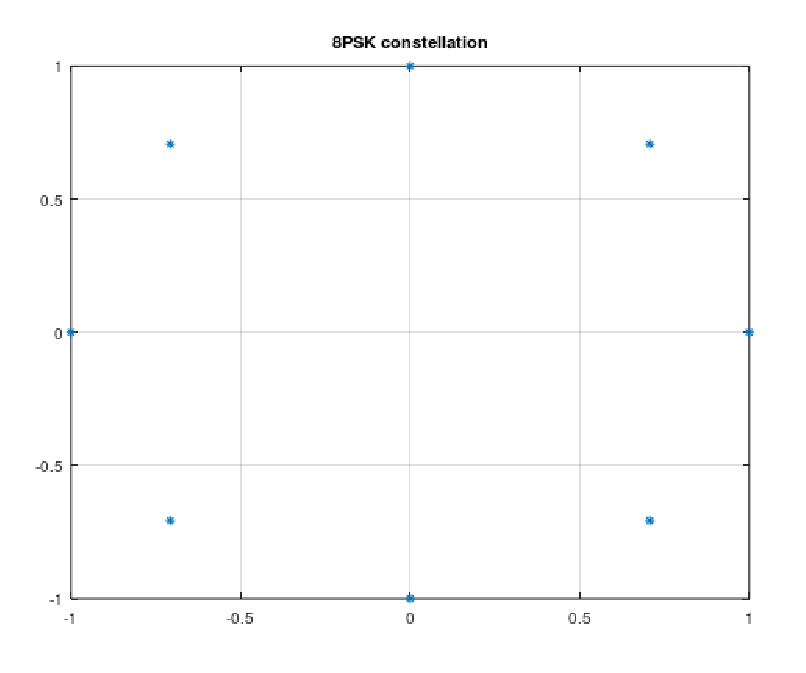
\includegraphics[width=\columnwidth]{./LMS_equalizer_octave/figs/psk.eps}
\caption{8-PSK constellation}
\label{fig:psk}
\end{figure}

\begin{figure}[!ht]
\centering
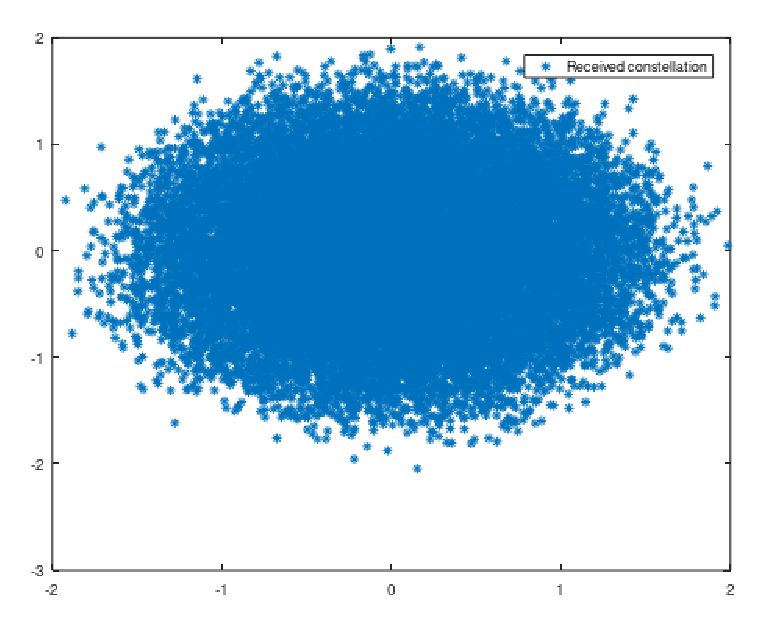
\includegraphics[width=\columnwidth]{./LMS_equalizer_octave/figs/constellation.eps}
\caption{Recieved constellation from the channel}
\label{fig:lms_mse}
\end{figure}

\begin{figure}[!ht]
\centering
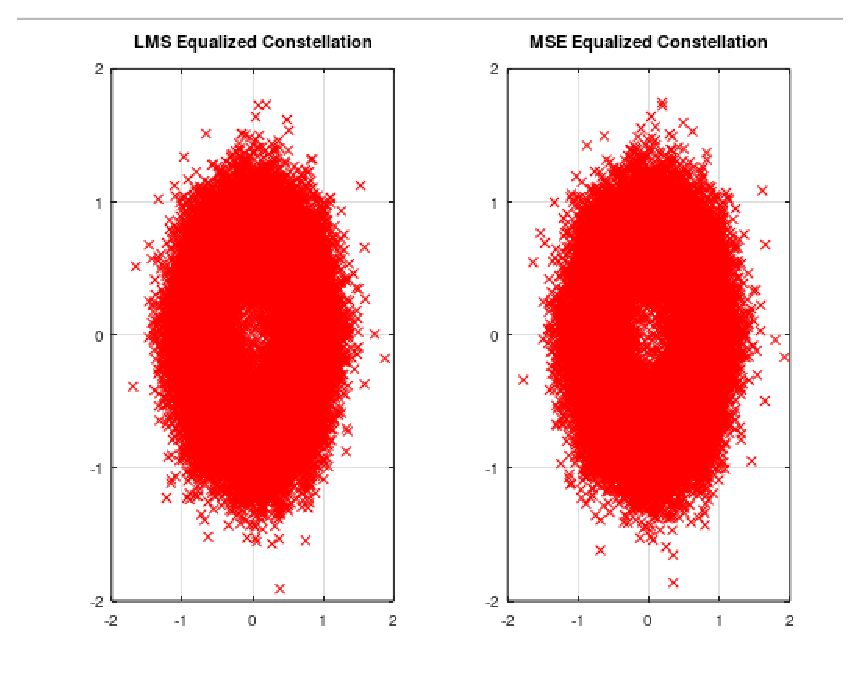
\includegraphics[width=\columnwidth]{./LMS_equalizer_octave/figs/lms.eps}
\caption{LMS and MSE equalized constellation}
\label{fig:lms_mse}
\end{figure}
Hence the code has been executed in octave.


\section{Frequency Offset: LR Technique}
%There are two parts.
%\begin{itemize}
%\item Estimate
%\item Exact
%\end{itemize}
Let the frequency offset be 
$\Delta f$  
\cite{freq_offset}
.  Then
\begin{align}
\label{eq:freq_offset_model}
\vec{y}_k= \vec{x}_k e^{j2\pi\Delta fkT_s} + \vec{n}_k, \quad k = 1,\dots,N 
\end{align}  
where $T_s \le \frac{1}{2\Delta f}$ is the sampling time.

\begin{equation}
\label{eq:freq_offset_model}
Y_k= X_k e^{j2\pi\Delta fkM} + V_k, \quad k = 1,\dots,N 
\end{equation}  
From \eqref{eq:freq_offset_model},
%
\begin{align}
Y_kX_k^*&= \abs{X_k}^2e^{j2\pi\Delta fkM}+ X_k^*{V}_k\\
\implies r_k&=e^{j2\pi\Delta fkM}+ \bar{V}_k
\end{align}
where
\begin{align}
r_k=Y_kX_k^*, \bar{V}_k=X_k^*{V}_k, \abs{X_k}^2=1
\end{align}
%
The autocorrelation can be calculated as
\begin{equation}
R(k) \overset{\Delta}{=} \frac{1}{N-k}\sum_{i=k+1}^{N} r_{i}r^{*}_{i-k}
 , 1 \leq k \leq N-1
\end{equation}
Where N is the length of the received signal.
%DVB-S2 operating with large frequency. So Large frequency offset model has to be employed which is the  Exact approximation of LR technique \cite{1}
For large centre frequency, the following yields a good approximation for frequency offset upto 40 
MHz.
\begin{equation}
\Delta\hat{f} \approx \frac{1}{2\pi M}\frac{\sum_{k=1}^{P}\text{Im}(R(k))}{\sum_{k=1}^{P}k\text{Re}(R(k))},
\quad  P\Delta{f}M << 1
\label{eq:Z}
\end{equation}
%
where $P$ is the number of pilot symbols.
\subsection{Plots}
%\begin{figure}
%\begin{center}
%\includegraphics[width=\columnwidth]{./figs/frequency_best.eps}
%\end{center}
%\caption{Error variation with respect to frequency offset.  }
%\label{fig:freq_best}
%\end{figure}
%%
%\begin{figure}
%\begin{center}
%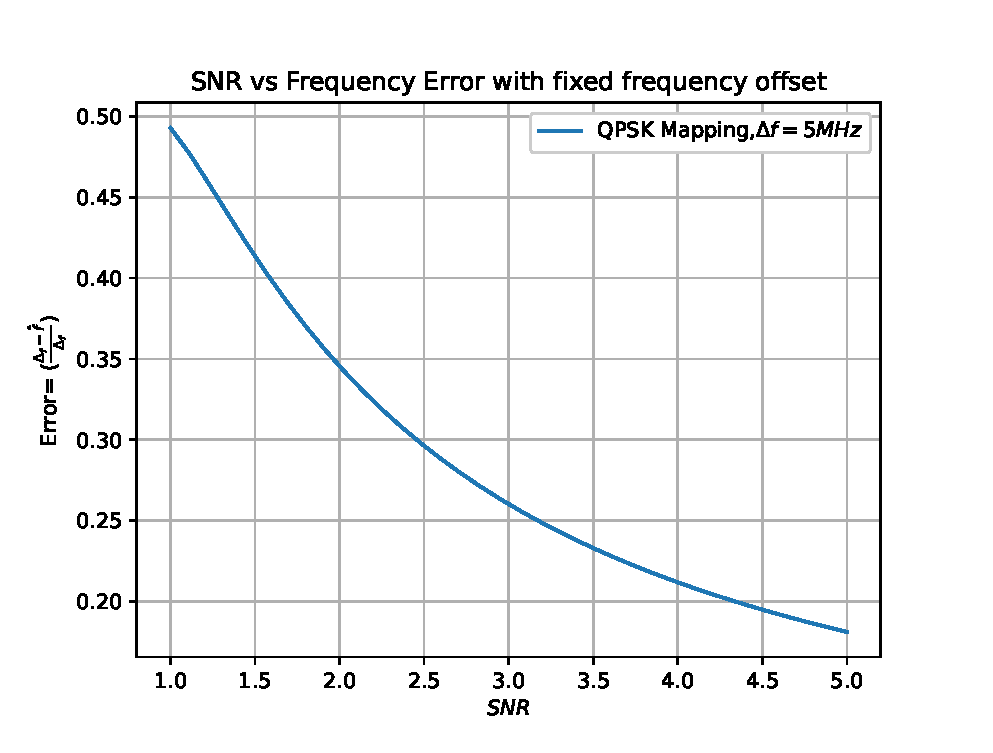
\includegraphics[width=\columnwidth]{./figs/frequencyestiamtion_best_error_vs_snr.eps}
%\end{center}
%\caption{Error variation with respect to the SNR.  $\Delta f = 5$ MHz, Center frequency $f_c=25$ GHz}
%\label{fig:freq_est}
%\end{figure}

%
The number of pilot symbols is $P = 18$. The codes for generating the plots are available at

Fig. \ref{fig:freq_best} shows the variation of the error in the offset estimate with respect to the offset 
$\Delta f$ when the SNR = 10 dB.  Similarly Fig. \ref{fig:freq_est} shows the variation of the error with 
respect 
to the SNR for $\Delta f = 5 $MHz.


%\section{QPSK}
%\subsection{Modulation}
\begin{enumerate}[label=\thesubsection.\arabic*.,ref=\thesubsection.\theenumi]
\numberwithin{equation}{enumi}
\numberwithin{figure}{enumi}



\item See Fig. \ref{fig:ee18btech11012_fig1} for the constellation diagram.  The transmitted symbol set is given by 
\begin{align}
\vec{s}_m = \myvec{\cos \frac{2m\pi}{8}\\ \sin \frac{2m\pi}{8}}, \quad m \in \cbrak{0, 1, \dots, 3}.
%\textbf{y = s + n}
\end{align}
%
The numerical values for $\vec{s}_m$ are listed in Table \ref{table: }
\begin{figure}[!ht]
                \resizebox{\columnwidth}{!}{
\begin{tikzpicture}

\draw[<->,thick] (-4,0)--(4,0) node[right]{$\phi_1$};
\draw[<->,thick] (0,-4)--(0,4) node[above]{$\phi_2$};

\filldraw[black] (2.5,0) circle (2pt) node[below] {$s_0$} ;
\filldraw[black] (0,2.5) circle (2pt) node[left] {$s_1$} ;
\filldraw[black] (-2.5,0) circle (2pt) node[below] {$s_2$} ;
\filldraw[black] (0,-2.5) circle (2pt) node[left] {$s_3$} ;

\end{tikzpicture}
}
\label{fig:ee18btech11041_fig1}
\caption{constellation diagram}
\end{figure}

%
\item See Table \ref{table: } for the encoding scheme.
\end{enumerate}
\subsection{Demodulation}
\begin{enumerate}[label=\thesubsection.\arabic*.,ref=\thesubsection.\theenumi]
\item The received symbol is then obtained as
\begin{align}
\vec{y} = \sqrt{E_s}\vec{s} + \vec{n}
\end{align}
%
where $E_s$ is the symbol energy and 

\begin{align}
\vec{n} &\sim \mathcal{N}\brak{\vec{0},\frac{N_0}{2}\vec{I}}
\\
\vec{s} &\in \cbrak{\vec{s}_m}_{m = 0}^{3}
\end{align}
\item The decision rule is given by Fig. \ref{fig:ee18btech11012_fig2} and can be expressed as







\begin{figure}[!ht]

                \resizebox{\columnwidth}{!}{
\begin{tikzpicture}

\draw[<->,thick] (-4,0)--(4,0) node[right]{$y1$};
\draw[<->,thick] (0,-4)--(0,4) node[above]{$y2$};
\draw [dashed]   (-4,-4)--(4,4);
\draw [dashed]   (-4,4)--(4,-4);

\filldraw[black] (2.5,0) circle (2pt) node[below] {$s_0$} node[above] {00};
\filldraw[black] (0,2.5) circle (2pt) node[left] {$s_1$} node[right] {01};
\filldraw[black] (-2.5,0) circle (2pt) node[below] {$s_2$} node[above] {11};
\filldraw[black] (0,-2.5) circle (2pt) node[left] {$s_3$} node [right] {10} ;

\foreach \coordinate/\label/\pos in {{(3,1)/D1/above left},{(1.5,3)/D2/right},{(-3,-2)/D3/above right},{(-1.5,-3)/D4/above right}} \node[\pos] at \coordinate {\label};

\end{tikzpicture}
}

\label{fig:ee18btech11041_fig2}
\caption{decision regions}
	
\end{figure}

Let \textbf{r} be the received bits, \textbf{r} = [$r_1$,$r_2$]. 
\begin{align}
    r_1 = 
    \begin{cases}
    0, &  \textbf{y} \in D1\cup D2 \Longleftrightarrow  y_1 + y_2 > 0\\
    1, &  \textbf{y} \in D3\cup D4 \Longleftrightarrow  y_1 + y_2 < 0
    \end{cases}
    \label{eq:ee18btech11041_eq1}
\end{align}

\begin{align}
    r_2 = 
    \begin{cases}
    0, &  \textbf{y} \in D1\cup D4 \Longleftrightarrow  y_2 - y_1 < 0\\
    1, &  \textbf{y} \in D2\cup D3 \Longleftrightarrow  y_2 - y_1 > 0
    \end{cases}
    \label{eq:ee18btech11041_eq2}
\end{align}

From eq.\ref{eq:ee18btech11041_eq1} and eq.\ref{eq:ee18btech11041_eq2}
\\
For detecting $s_0$, $y_1 > -y_2$ and $y_1 > y_2$.
\\
For detecting $s_1$, $y_1>-y_2$ and $y_1<y_2$.
\\
For detecting $s_2$,  $y_1<-y_2$ and $y_1<y_2$.
\\
For detecting $s_3$, $y_1<-y_2$ and $y_1>y_2$.




\item The following code has simulation of QPSk.
\begin{lstlisting}
 codes/qpsk.py
\end{lstlisting}

\end{enumerate}


\bibliography{IEEEabrv,Theresh_timesync.bib}
\end{document}


